%\documentclass[lineno,twocolumn,endfloat]{biophys-new}
\documentclass{biophys-new}
\usepackage[utf8]{inputenc}
\usepackage{graphicx}
\usepackage[colorlinks,allcolors=cyan!70!black]{hyperref}
\usepackage{lipsum}
\usepackage{xcolor}
\usepackage[version=3]{mhchem}
\usepackage{gensymb}
\usepackage{amsmath,amsfonts,amssymb,amsthm,mathtools} % AMS
\usepackage{listings}

\title{ Wavelet analysis reveals coherence dynamics between trigerred and spontaneous \ce{Ca^2+} oscillations in subepicardial cardiomyocytes }
\runningtitle{Calcium waves wavelet analysis} %% For page header
\author[1,*]{Danila Bobkov}
\author[7]{Galina Sakuta}
\author[3]{Ekaterina Baidyuk}
\author[4]{Andrei Stepanov}
\author[5]{Igor Kubasov}
\author[6]{Maxim Dobretsov}
\author[7]{Sandor Gyorke}
\runningauthor{Bobkov et al.} %% For page header
\affil[1,2,3]{Institute of Cytology of the Russian Academy of Science, 194064 Tikhoretsky ave. 4, St-Petersburg, Russia}
\affil[4,5,6]{Sechenov Institute of Evolutionary Physiology and Biochemistry of the Russian Academy of Science, 194223 Russia Saint-Petersburg pr.Torez 44}
% \affil[6]{Department of Anesthesiology, University of Arkansas for Medical Sciences, Little Rock, AR, United States}
\affil[7]{Dorothy M. Davis Heart and Lung Research Institute, College of Medicine, Ohio State University, Columbus, OH, United States}
\corrauthor[*]{dan.bobkov@gmail.com}
\papertype{Article}

\begin{document}
\begin{frontmatter}
\begin{abstract}


 This study examines the changes in \ce{Ca^2+} oscillations frequencies which begin
 ical implications in a model of
 an additional strong damage factor during reperfusion is the occurrence of
\ce{Ca^2+} ions play a key role in the electrical and mechanical responses of the heart.
With a deficiency of ATP caused by hypoxia,
With a deficiency of ATP caused by hypoxia, cardiomyocytes are damaged, with the formation of necrotic striation.
Sporadic \ce{Ca^2+} waves was observed using confocal laser microscopy in the subepicardial layers of the myocardium of an isolated rat heart under hypoxic conditions.
Such waves propagate a short distance around their source and interfere with sinus rhythm.
We identified high-frequency \ce{Ca^2+} oscillators, that arise in cardiomyocytes at the sites of local damage caused by hypercontraction.
The source of these waves are local \ce{Ca^2+} release regions, associated with hypercontraction damage sites.
High-frequency oscillations are non stationary in their nature, and temporal understanding is dynamics of their spectral characteristics is
Analysis of the frequency and amplitude characteristics of calcium waves in made it possible to characterize them as damped oscillations with maximum frequency of about 3 Hz with damping rate of about 0.27 Hz/min.
Wavelet coherency analysis revael that high-frequency \ce{Ca^2+} oscillators can interfere with the third and second harmonics of sinus rhythm, leading to the presence of time intervals with increased coherence between the aberrant and normal rhythm.
These data imply that in failing cardiomyocyte can be autonomous
The findings suggest possible involvement of abnormal \ce{Ca^2+} release from the sarcoplasmic reticulum in the process of arrhythmogenic activity of the heart in hypoxic condition.



\textit{Key words:} calcium waves, cardiomyocytes, myocardium, ischemia, arrhytmia, wavelet coherence

\end{abstract}
\end{frontmatter}

\section*{Introduction}

Integral \ce{Ca^2+} release from the sarcoplasmic reticulum following action potentials propagating along the excitable membrane of cardiomyocytes is the main factor initiating a contractile response.
Arrhythmias associated with myocardial damage are one of the leading causes of death in the ageing human population (\cite{xiao2011cardiac}, \cite{}).
An intracellular accumulation of \ce{Ca^2+} caused by a failure of the ATP-dependent mechanisms known to be the key events in myocardial damage during ischemia \cite{shen1972myocardial,shen1972kinetics,nayler1981role}.
In the process of damage progression functional myocardial tissue becomes \ce{Ca^2+}-overloaded and then lost functionality with the properties of \ce{Ca^2+} waves changing progressively over time \cite{minamikawa1997situ,hama1998real}.
Under a number of adverse conditions and/or according to individual heart diseases, abnormal forms of \ce{Ca^2+} release from the sarcoplasmic reticulum are observed, which may cause arrhythmogenesis \cite{ishide1990propagation}.
One form of this abnormal release is spontaneous space-time changes in the level of \ce{Ca^2+} in the cytoplasm (sporadic \ce{Ca^2+} waves), observed both in isolated cardiomyocytes (2, 3) and in situ experiments, including the perfused heart (4, 5).
However, the sources of these waves, the conditions for their appearance, as well as their role and influence on the heart muscle, are not well understood.
It is known that hypoxia of the heart muscle is often accompanied by tachycardia, group extrasystoles, bouts of paroxysmal rhythm disturbances.
The extent to which these violations can be associated with the appearance of \ce{Ca^2+} waves remains unknown.
\ce{Ca^2+} dynamics at the border zones between the infarcted and non-infarcted myocardium is considered to be a key element for arrhythmogenesis \cite{takamatsu2008arrhythmogenic}.
The aim of the work was to find out whether hypoxia as one of the factors of myocardial damage can trigger sporadic \ce{Ca^2+} waves, and if so, can these waves affect the oscillatory activity of intact cardiomyocytes in the working heart.
We applied the method of confocal microscopy and carried out a frequency analysis of calcium oscillations in cardiomyocytes from border zone between the necrotic and healthy myocardium.


CICR and sinus rhythm
Measurement of \ce{Ca^2+} waves in isolated rat heart
Now it is well acknowledged that \ce{Ca^2+} - overloaded cardiomyocytes are essential substrate for arrhythmias and contractile failure, especially in acute myocardial infarct.
In this study,
Wavelet tranform of electrocardiogram (ECG) ECG-derived data \cite{sharma2017use}
For optical registration of calcium waves \cite{matsuura2018intravital} ...
Here we provide an approach for investigation the spatio–temporal frequency domains in multicellular speciemen.
Unstationarity in Calcium Oscillations in Isolated Heart Revealed by Wavelet Analysis
Spectral analysis of hypoxia-indused calcium waves in isolated rat heart on the subcellular level reveal local hypercontraction sites as sources for hight-frequency oscillations.
Local hypercontracts are centers of high-frequency calcium oscillations
damage progression line

\section*{Materials and Methods}

\textcolor{red}{Capitalize trade names and give manufacturers full names and addresses (city and state).}

\subsection*{Animals}

Studies were conducted in accordance with regulations of the National Committee on Bioethics of the Russian Academy of Sciences.
The protocol was approved by the Ethics Committee of the Sechenov Institute of Physiology and Evolutionary Biochemistry.
Experiments were performed in hearts isolated from adult Wistar male rats (N = 00; body weight 200–250 g).

\subsection*{Heart staining}

Animals were anesthetized with sodium Nembutal (50 kg - 1 , i.p., 50 mg), and then the hearts were harvested/removed via thoracotomy.
The preparation was retrogradely perfused via the aortic cannula through with a Tyrode’s solution of the following composition (mM): 140 NaCl, 1.0 \(\,\mathrm{Mg}\mathrm{Cl}_2\), 4.5 \ce{KCl}, 10 glucose, 1 \ce{CaCl2} and 10 HEPES.
The pH of the solution was maintained at 7.4 by continuously bubbling with 95\% \ce{O2}/ 5\% \ce{CO2} and temperature maintained at 37 C\degree.
Effluent was drained via a catheter placed in dish so as not to touch the heart.
Myosin ATPase inhibitor, blebbistatin (10 $\mu$M, Sigma, USA) was added to the Tyrode’s solution perfusing the heart to stop heart contraction and prevent associated artifacts (Farman et al., 2008).
To prevent motion artifact in optical recordings, muscle contraction was inhibited with 20 $\mu$ M/L of (-)-blebbistatin \cite{kong2014role}.
The dyes Fluo-4-AM,Tetramethylrhodamine Methyl Ester Perchlorate, TMRM, and Di-8-ANEPPS, was obtained from Thermo Fisher Scientific.
Heart perfusion was performed using a modified Langendorff system. Tyrode solution with \ce{CaCl2} (1 mM/L) was used as the perfusion medium.
A similar solution with the addition of the fluorescent dyes Fluo-4 (20 $\mu$ M/L) and Di-8-ANEPPS (20 $\mu$ M/L) was used for visualization of the \ce{Ca^2+} waves.


\subsection*{Confocal microscopy}
To investigate spontaneous \ce{Ca^2+} waves in myocardium, we positioned isolated perfused heart in organ bath with thin bottom (180 $\mu$ m), left ventricle in conjunction with an oil-immersible objective lens on an inverted microscope (Leica).
This combination provide sufficient depth discrimination to focus directly onto the epicardial layers and individual cells within the intact functioning organ.

To the simultaneous detection of fluorescence of Fluo-4 and TMRM we used an argon laser with a wavelength 488 nm and a power of 80\% and a HeNe laser with a wavelength of 543 nm and a power of 80\%. The fluorescence detection was carried out in the spectral range 493 nm -- 540 nm for Fluo-4 and 552 nm -- 792 nm for TMRM. Since the specific values of the background fluorescence depended on the density of the capillary network, the amount of connective tissue in the field of view, and other factors, the sensitivity of the PMT detector (gain) was selected individually each time, depending on the conditions of the survey, and was usually 600 to 800 units.
changes in fluorescence intensity of Fluo-4 over time (xyt mode) were measured, a resonant scanner (8000 Hz) was used, and the diameter of the confocal pinhole was set to 100 $\mu$m.
A fluorescent signal was registered in the first layer of cardiomyocytes adjacent to the epicardial surface of an isolated heart (Fig. 1). The fluorescent signal was measured in a whole frame or in certain regions of interest (regions of interest, ROI).
Spectral analysis of calcium oscillations was carried out using a fast Fourier transform.
Studies were carried out on the model of an isolated working rat heart perfused by the method of Langendorff.
The subepicardial layers of the myocardium were examined using an inverted Leica TCS SP5 laser scanning confocal microscope equipped with a resonance scanner and x10, x20, x63 lenses with oil immersion.
For visualization of cardiomyocytes, vascular network and connective tissue, perfusion of the hearts was performed with a solution with the addition of the fluorescent dye Di-8-ANEPPS.
To visualize free \ce{Ca^2+} ions, the Fluo-4 dye was used.
For dyeing mitochondria, the TMRM dye was used, the fluorescence intensity of which is proportional to the value of the mitochondrial membrane potential ( $\Delta\psi$).
With the simultaneous detection of fluorescence Fluo-4 and Di-8-ANEPPS, an argon laser with a wavelength of 488 nm and a power of 80\% was used to excite the fluorescence.
Fluorescence detection was carried out using two photomultiplier tubes (PMT), 491nm - 581nm for Fluo-4 and 611nm - 792nm for Di-8-ANEPPS.
With the simultaneous detection of fluorescence Fluo-4 and TMRM, an argon laser with a wavelength of 488 nm and a power of 80\% and a HeNe laser with a wavelength of 543 nm and a power of 80\% were used to excite the fluorescence.
The fluorescence detection was carried out in the spectral range 493 nm-540 nm for Fluo-4 and 552 nm --- 792 nm for TMRM.
Since the specific values of the background fluorescence depended on the density of the capillary network, the amount of connective tissue in the field of view, and other factors, the sensitivity of the PMT detector (gain) was selected individually each time, depending on the conditions of the survey, and was usually 600 to 800 units.
For optical registration of calcium waves, changes in fluorescence intensity of Fluo-4 over time (xyt mode) were measured, a resonant scanner (8000 Hz) was used, and the diameter of the confocal pinhole was set to 100 $\mu$m.
A fluorescent signal was registered in the first layer of cardiomyocytes adjacent to the epicardial surface of an isolated heart (Fig. 1). The fluorescent signal was measured in a whole frame or in certain regions of interest (regions of interest, ROI).
Spectral analysis of calcium oscillations was carried out using a fast Fourier transform.
Calcium imaging with Fluo-4/AM was performed using a confocal laser scanning microscope Leica SP5 with a 40x (NA = 1.3) oil immersion objective. Fluorescence images (excited at 488 nm).
The pinhole was set to 200 mm, resulting in , 2.5-mm optical slices. Amplifier gain and detector offset were adjusted such that neither saturation nor threshold cutoff occurred.
The membrane structure of epicardial myocytes was analyzed in situ by confocal microscopy Leica SP5 equipped with x63 (NA = 1.4) oil-immersion lens]. The epicardial images were used to define the

\subsection*{Data collection and analysis}

\textcolor{red}{In addition, you can use }
\verb|\ref{...}| and \verb|\label{...}| commands for cross-references.

\begin{table}[hbt!]
\caption{An example table}
\label{tab:widgets}
\centering
\begin{threeparttable}
\begin{tabular}{c l r f}
\hline
Code & Item & Quantity & Square, $\mu m^2$  \\\hline
40 cells\tnote{b} & Cells & 40 & 1\tnote{a}  \\
24x24 grid & ROIs & 576 & 318.2656   \\
\hline
\end{tabular}
\begin{tablenotes}
\item[a] Mean ROI square.
\item[b] Manully selected.
\end{tablenotes}
\end{threeparttable}
\end{table}


Recorded time-series image stack were analyzed in ImageJ v.1.52p software\cite{rueden2017imagej2}.
measurement duration= 109.6 s sampling frequency 14.29745 Hz
Time series analysis in BAR plugin: raw signal and
normalization against F0, multi ROI profiler


Frequency estimation usig Fast Fourier Transform with Hamming window --- available as spectrogram function in phonTools package.

576 ROI 17.84 x 17.84 $\mu$m were selected using ImageJ macros (see Supplementary\ref{macros})
Wavelet analysis
Formula from \cite{grinsted2004application} and from \cite{kahraman2016multiple} ...
To cite R in publications use:  \cite{team2014r}

To cite package WaveletComp in publications use: \cite{rosch2016waveletcomp}
Wavelet methodology is a reasonable choice to study periodic phenomena in time series, particularly in
the presence of potential frequency changes across time.
packages for wavelet analysis in R
number of simulations = 100
WaveletComp (version 1.1) analyzes the frequency structure of uni- and bivariate time series using the Morlet wavelet.
This wavelet leads to a continuous, complex-valued wavelet transform of the time series withy careful selection of time and frequency resolution parameters. The transform provides information on both local amplitude and instantaneous phase of any periodic process across time with subsequent investigation of coherency between two time series.


The “mother” Morlet wavelet is:
\begin{equation}\label{eq:morlet}
\psi(t)=\pi^{-1/4}e^{i\omega t-{t^2}/2}
\end{equation}


In formula~\ref{eq:morlet} “angular frequency” $\omega$ is set to 6 since it makes the Morlet wavelet approximately analytic.
The Morlet wavelet transform of a time series (${x}_{t}$) is defined as the convolution of the series with a set of “wavelet daughters” generated by the mother wavelet by translation in time by $\tau$ and scaling by \textit{s}:
\begin{equation}\label{eq:wave}
\text{Wave}(\tau, s)=\sum_{t}x_{t}\frac{1}{\sqrt{s}}\psi^{\ast}\left(\frac{t-\tau}{s}\right)
\end{equation}

In formula~\ref{eq:wave} $\tau$ is the localizing time parameter defines position of the particular daughter wavelet in the time domain, and the set of scales $s$ determines the wavelet coverage of the series in the frequency domain.
WaveletComp uses Fast Fourier Transform algorithms to evaluate formula~\ref{eq:wave} efficiently.
The evolving in time local amplitude of any periodic component of the time series can then be retrieved from the modulus of its wavelet transform with rectification:
\begin{equation}\label{eq:amplitude}
\text{Ampl}(\tau, s)=\frac{|\text{Wave}(\tau, s)|}{\sqrt{s}}.
\end{equation}

The wavelet power spectrum is the square of the amplitude, understand as time-frequency (or time-period) wavelet energy density:
\begin{equation}\label{eq:power}
\text{Power}(\tau, s)=\frac{|\text{Wave}(\tau, s)|^2}{s}.
\end{equation}

Displacements of periodic phenomena relative to the localizing origin $\tau$, shifted across the time domain, are given by the instantaneous or local wavelet phase.
It can be wrapped to represent an angle in the interval $[-\pi,\pi]$:
\begin{equation}\label{eq:phase}
\text{Phase}(\tau, s)=\text{Arg}(\text{Wave}(\tau, s))=tan^{-1}\left(\frac{\text{Im}(\text{Wave}(\tau, s))}{\text{Re}(\text{Wave}(\tau, s))}\right).
\end{equation}

The concepts of cross-wavelet analysis provide appropriate tools for (i) comparing the frequency contents of two time series, (ii) drawing conclusions about the series’ synchronicity at certain periods and across certain ranges of time.
The cross-wavelet transform of two time series (x t ) and (y t ), with respective wavelet transforms Wave.x and Wave.y, decomposes the Fourier co- and quadrature-spectra in the time-frequency (or time-scale) domain.
WaveletComp implements the rectified version according to Veleda et al. [16]:
\begin{equation}\label{eq:wave.xy}
\text{Wave.xy}(\tau, s)=\frac{\text{Wave.x}(\tau, s)\cdot\text{Wave.y}^{\ast}(\tau, s)}{s}
\end{equation}

Its modulus can be interpreted as cross-wavelet power; it lends itself, with certain limitations, to an as-
sessment of the similarity of the two series’ wavelet power in the time-frequency (or time-scale) domain:
\begin{equation}\label{eq:power.xy}
\text{Power.xy}(\tau, s)=|\text{Wave.xy}(\tau, s)|
\end{equation}

Information about the two series’ synchronization in terms of the instantaneous or local phase advance of any periodic component of (x t ) with respect to the correspondent component of (y t ), viz. the so-called phase difference of x over y at each localizing time origin and scale:
\begin{equation}\label{eq:angle}
\text{Angle.xy}(\tau, s)=\text{Arg}(\text{Wave.xy}(\tau, s))
\end{equation}

This equals the difference of individual phases, Phase.x --- Phase.y, when converted to an angle in the
interval $[-\pi,\pi]$.
Phase differences are displayed as arrows in the image plot of cross-wavelet power.

In order to analyze displacements of periodic phenomena in two time series, a comparative plot of wavelet coherency may be helpful.
Wavelet coherency  measures the cross-correlation between two time series as a function of frequency: the wavelet coherence is given by the formula:
\begin{equation}\label{eq:coherence}
\text{Coherence}=\frac{|\text{sWave.xy}|^2}{\text{sPower.x}\cdot\text{sPower.y}}
\end{equation}
The need for smoothing is indicated by the prefix s.


Contour lines added to the wavelet power spectrum delineate areas of high significance.
Wavelet power spectrum of the series with variable period
Horizontal arrows pointing to the right indicate that the two series x and y are in phase at the respective period with vanishing phase differences.
Likewise, horizontal arrows pointing to the left indicate that the two series are in anti-phase;
The arrows are plotted only within white contour lines indicating significance (with respect to the null hypothesis of white noise processes) at the 10\% level.

10 simulations using analyze.wavelet function from WaveletComp package was run do plot Cross-Wavelet power spectrum of the series with interval color key and restricted arrow area.
Limit the area where arrows are drawn to the region where both individual wavelet transforms of x and y show significance (set which.arrow.sig = "wt"), and avoid the artifacts of the
The significance level of contour lines defined to . The plot of the ridge can be restricted to a high-level region ("high" according to a given level of plotted values). In particular, the area to be filled with arrows can be determined in several ways: to reflect significance (at a given level) with respect to cross-wavelet power, wavelet coherence, or individual wavelet power, and/or to flag a high-value region. Furthermore, there is an option to clear out the area where the p-values of cross-wavelet power (coherence, respectively) exceed a given level.

30 simulations was run to compute wavelet coherency.

Calibration with a sine wave signal
1 Hz and 5 Hz waves are represented in the picture \ref{waves are represented in the picture}
A Test Signal Containing Four Sequential Sinusoids


for 094--: 455.9 mkm / 512px = 0,8904296875
Area = 318,363, x = 17.8427296118, $\approx$ 17.84 $\mu$ m
analyze - tools - scale bar


\section*{Results and Discussion}

Calcium waves
How calcium waves are formed and what the consequences may be.
Solitons

coherence with its own main harmonic can be considered as an indicator of normality

\begin{figure}[hbt!]
\centering
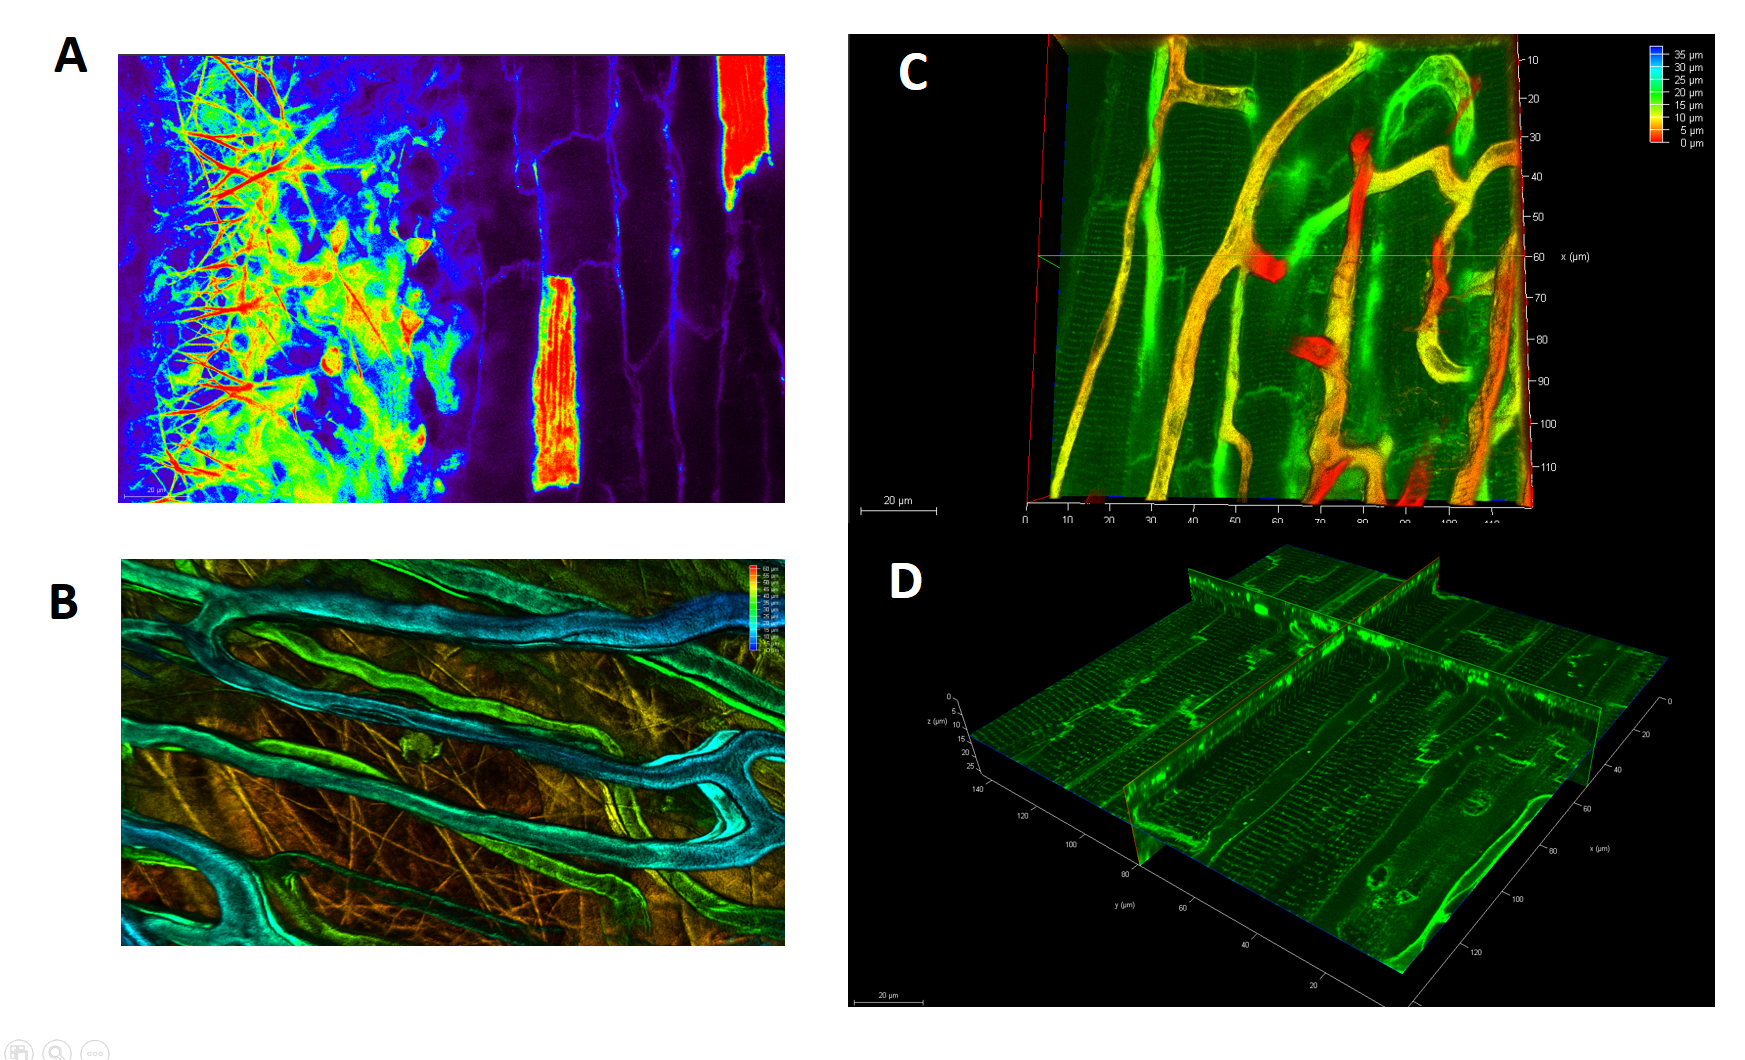
\includegraphics[width=0.8\linewidth]{fig1.png}
\caption{Confocal view in 10x objective of mitochondrial potential (red) and calcium (green) staining of epecardial cardiomyocytes in normal (A) and hypoxic (B) conditions. (C) Pseudocolor intensity imaging of Ca-overloaded cells and connective tissue in  tangential section of live hear wall. (D) 3D models of  cappillaries and characteristic section depth for calcium waves registration.}
\label{fig:fig1}
\end{figure}


\begin{figure}
    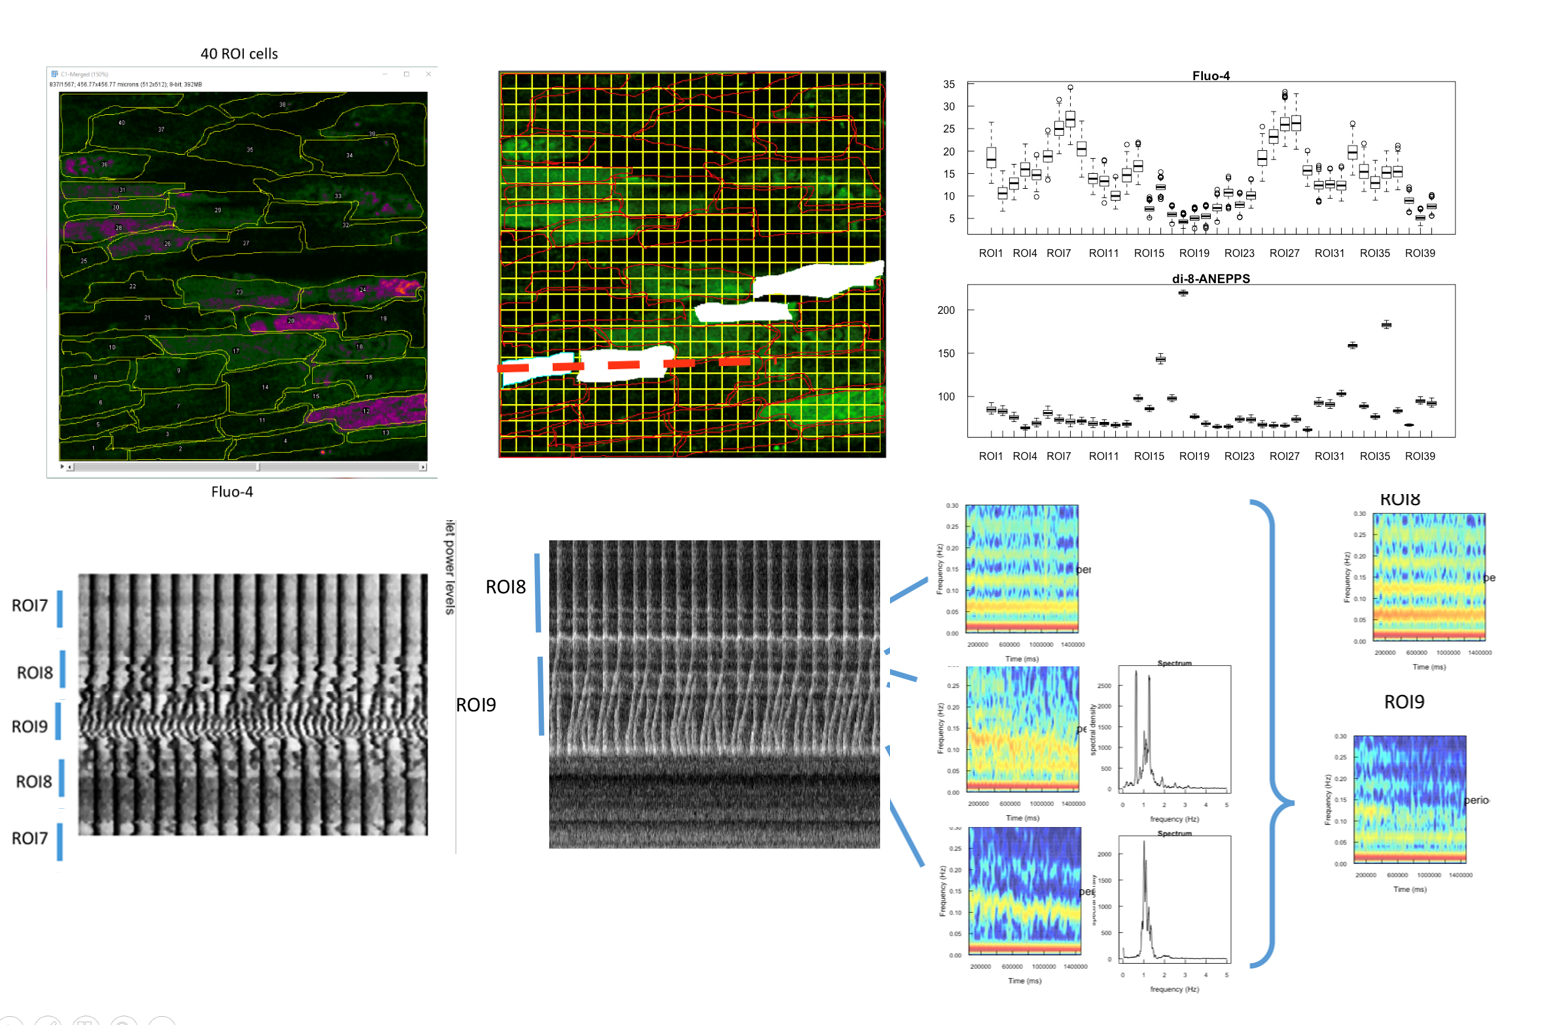
\includegraphics[width=0.8\linewidth]{fig2.jpg}
    \caption{Ischeamia induced LHFOCR}
    \label{fig:fig2}
\end{figure}

Plus video in good resolution in supplement. In futhure research we used 512 resolution for the sake of time resolutuon


\begin{figure}
    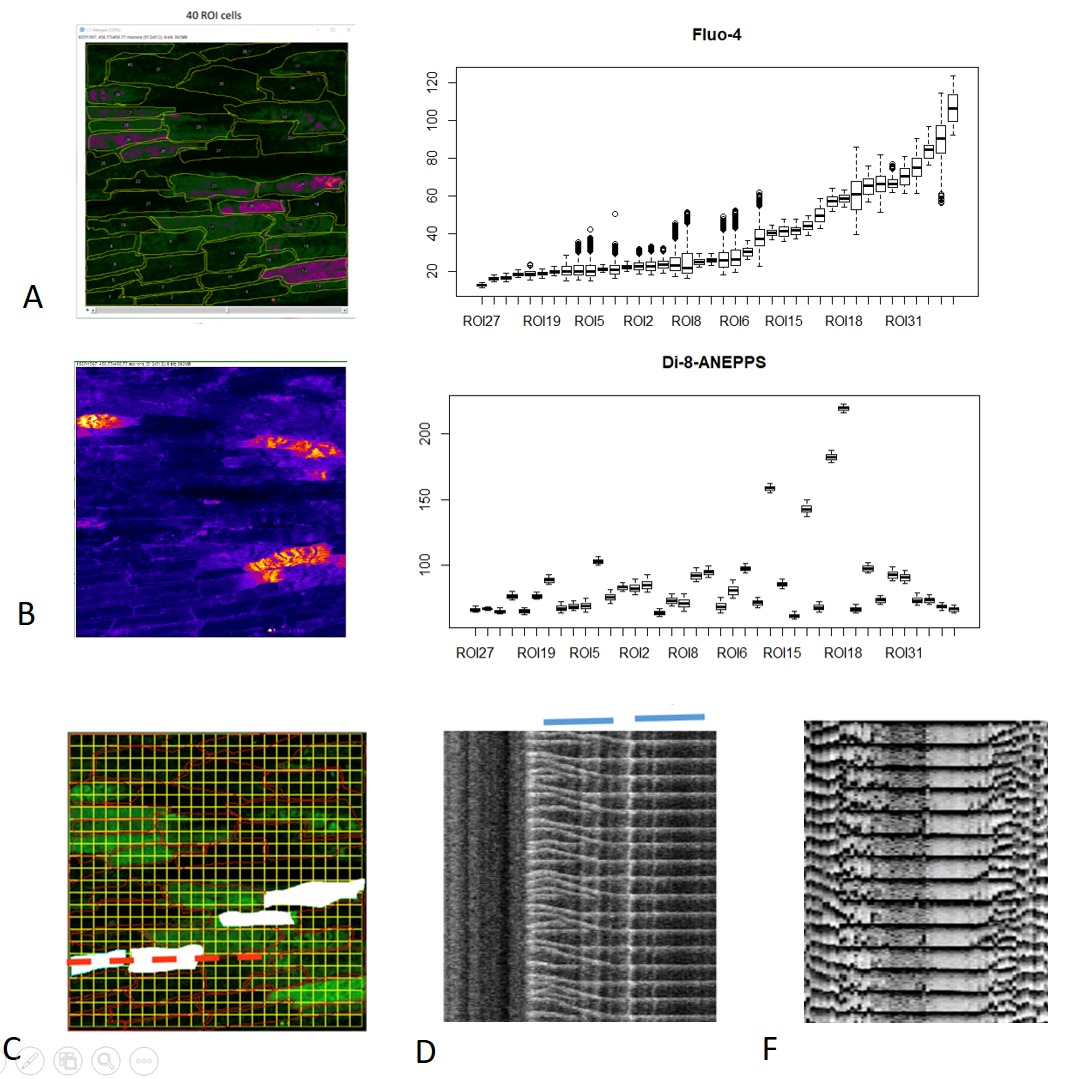
\includegraphics[width=0.9\linewidth]{fig3.png}
    \caption{(A) Fluo-4 raw image with 40 cells manually selected and  boxplots of collected signals ordered in according with ariphmetic mean; (B) 8-Di-ANEPPS signal image and boxplots of correspondent cells. (C) 24 x 24 ROI grid, dotted red line is region for kinesiogramm (D) and correspondent region from clustered heat map of signal from 24 x 24 ROI grid (F).}
    \label{fig:fig3}
\end{figure}


In ischemic myocardium, calcium waves are considered as an arrhythmogenic substrate.


\begin{table}[hbt!]
\caption{Frequency table}
\label{tab:freq}
\centering
\begin{threeparttable}
\begin{tabular}{c l r}
\hline
Code & Frequency & Amplitude  \\\hline
1st harmonic & 0.9025 & 3.2154 \\
2nd harmonic & 1.7960 & 1.4527  \\
3d harminic & 2.6984 & 0.5887    \\
\hline
\end{tabular}
\begin{tablenotes}
\end{tablenotes}
\end{threeparttable}
\end{table}


The effect of hypoxia on calcium oscillations in the epicardial layer of cardiomyocytes.


\begin{figure}
    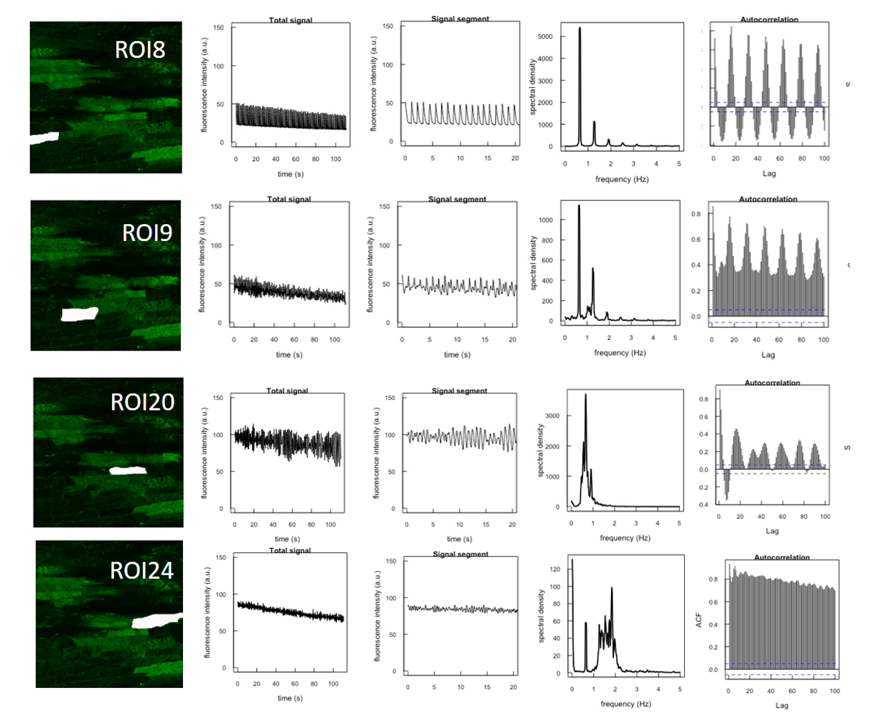
\includegraphics[width=0.9\linewidth]{fig4.png}
    \caption{(G) Normalized against F0 (left) and not normalized (right) frames with ROI selection and heat maps of manully selected ROI for wavelet analysis}
    \label{fig:fig4}
\end{figure}


In the course of myocardial observations after simultaneous staining of Di-8-ANEPPS and Fluo-4 under conditions where cardiac contractions were inhibited by blebbistatin, normal myocardial regions characterized by passage of a global calcium-ejection wave corresponding to sinus rhythm and small contractions were revealed. Tissue abbreviations were determined by averaging the Di-8-ANEPPS fluorescent signal from ten arbitrarily selected ROIs of 20 $\mu$ m x 20 $\mu$ m size (Figure 5). Also, the areas of the myocardium, located in different stages of ischemic damage, were identified. For the initial stage of damage, groups of cardiomyocytes with an increased value of \ce{Ca^2+}, in which high-frequency calcium waves were observed (Fig. 6), are characteristic. Nascent on the edge of the cell or in its middle, these waves can spread to neighboring cells (Figure 7). With a slight increase in the intracellular calcium concentration, such waves are erased by each subsequent global calcium release (Figure 11, B), and with a strong increase in \ce{Ca^2+} in cardiomyocytes relative to the baseline observed in the normal myocardium, the global calcium release does not interfere with the formation of calcium waves (Fig. 11, B, D). The cardiomyocytes adjacent to the necrosis zone were characterized mainly by slow, damped calcium waves with a large amplitude (Fig. 8).


\begin{figure}
    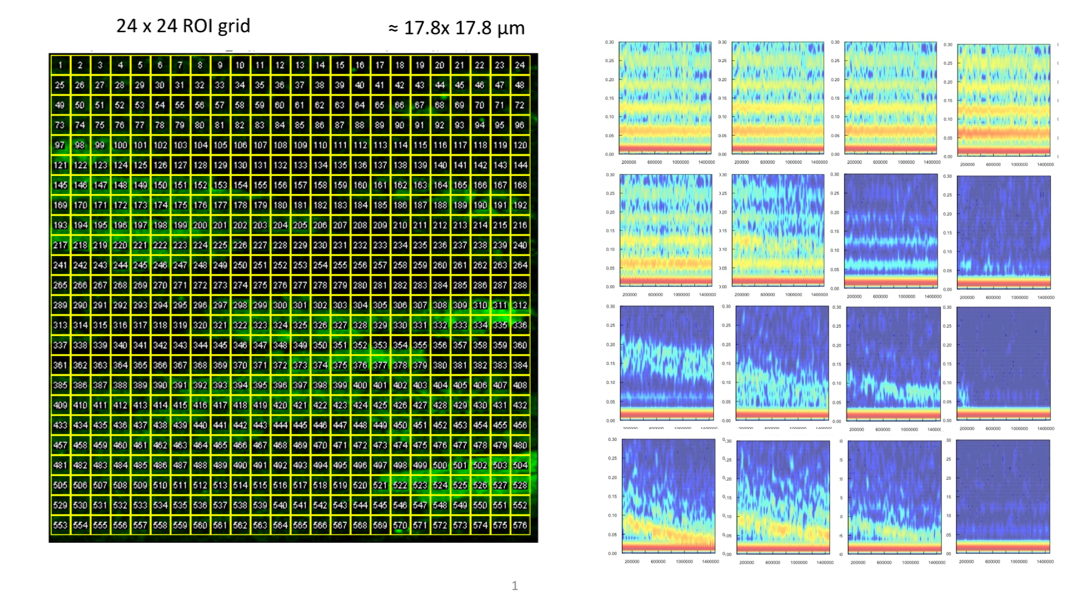
\includegraphics[width=0.9\linewidth]{fig5.png}
    \caption{Calibration with 1 Hz sin wave, Time series analysis and wavelet coherence , We used a non-stationary artificial signal with three data regions each containing a sinusoid of different frequency.}
    \label{fig:fig5}
\end{figure}


Calcium waves in the subepicardial myocardium in Langendorff-perfused rat heart.
We found that cardiomyocytes located in the border zone adjacent to the necrosis zone are characterized by an increased content of \ce{Ca^2+} ions, a reduced mitochondrial potential and contractile activity.


\begin{figure}
    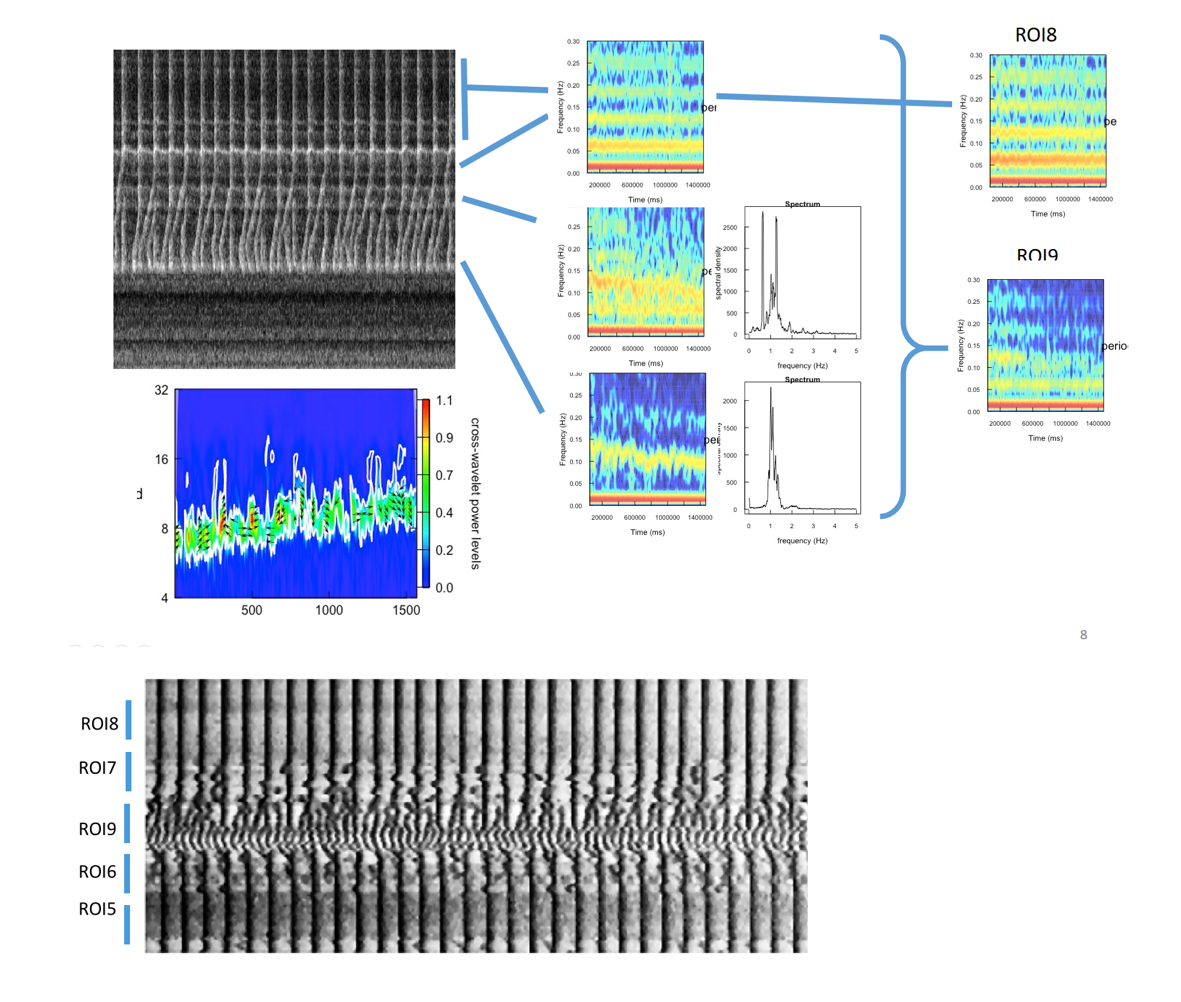
\includegraphics[width=0.9\linewidth]{fig6.png}
    \caption{Coherence of ANEPPS with 0.9 Hz sin wave }
    \label{fig:fig6}
\end{figure}



\begin{figure}[hbt!]
\centering
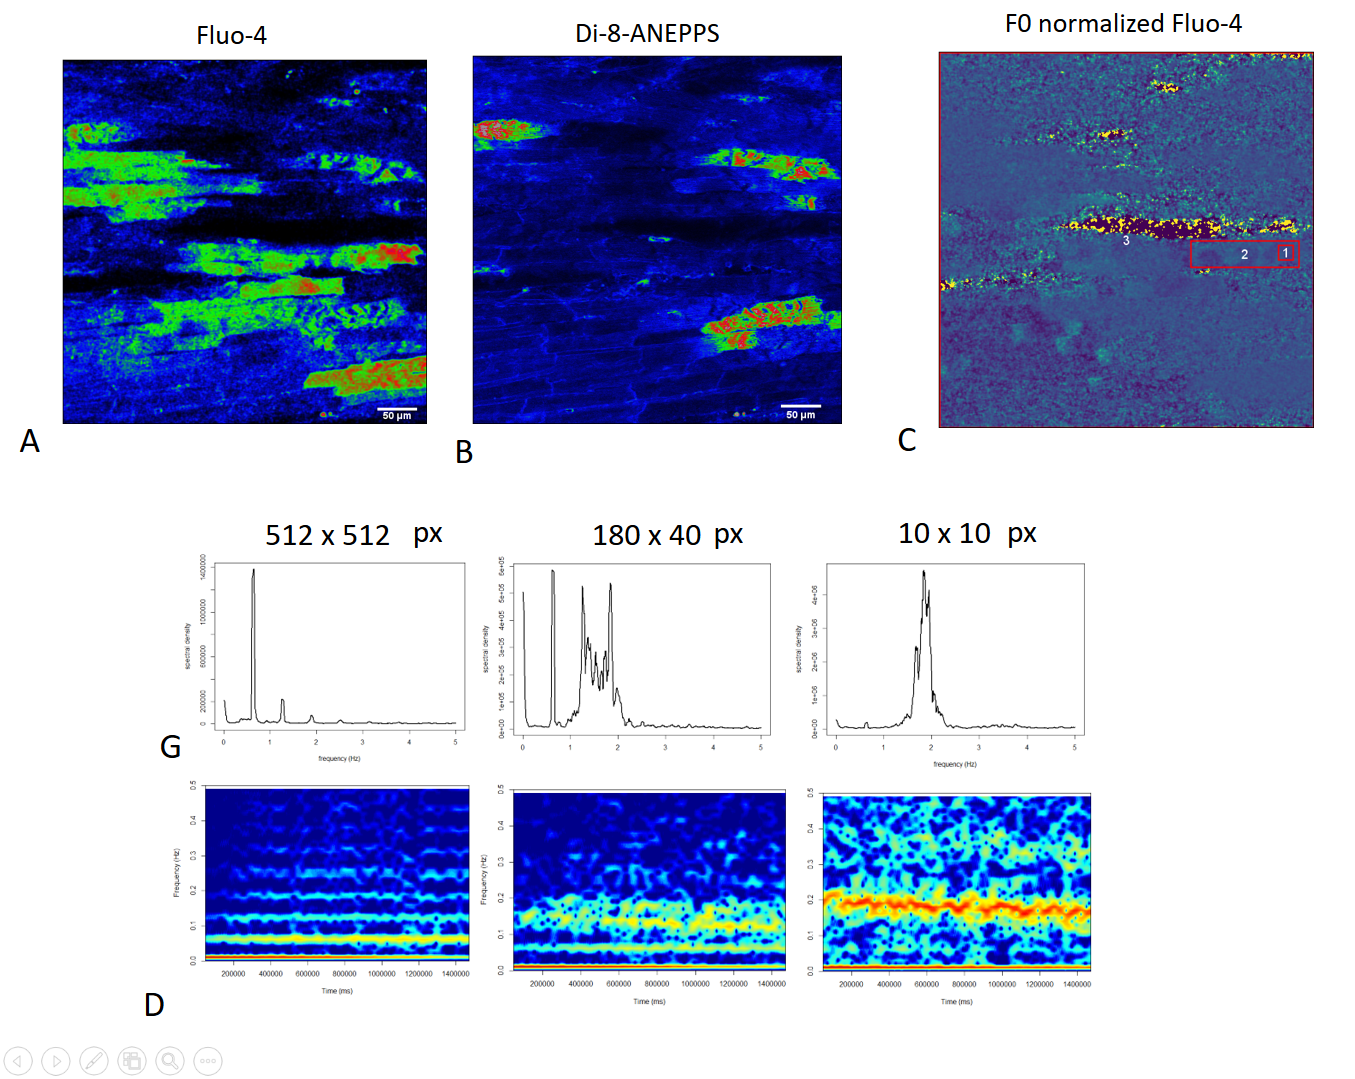
\includegraphics[width=0.9\linewidth]{fig7.png}
\caption{Flou-4 fluorescence intensity signals Nested ROI with the appropriate pixel dimensions: 512x512 - whole frame, 180x40 - one cell, 40x40,10x10, 2x2 - cell areas containing HFOLS. }
\label{fig:fig7}
\end{figure}


Simultaneous recordings of AP-induced and spontaneous calcium transients

\begin{figure}[hbt!]
\centering
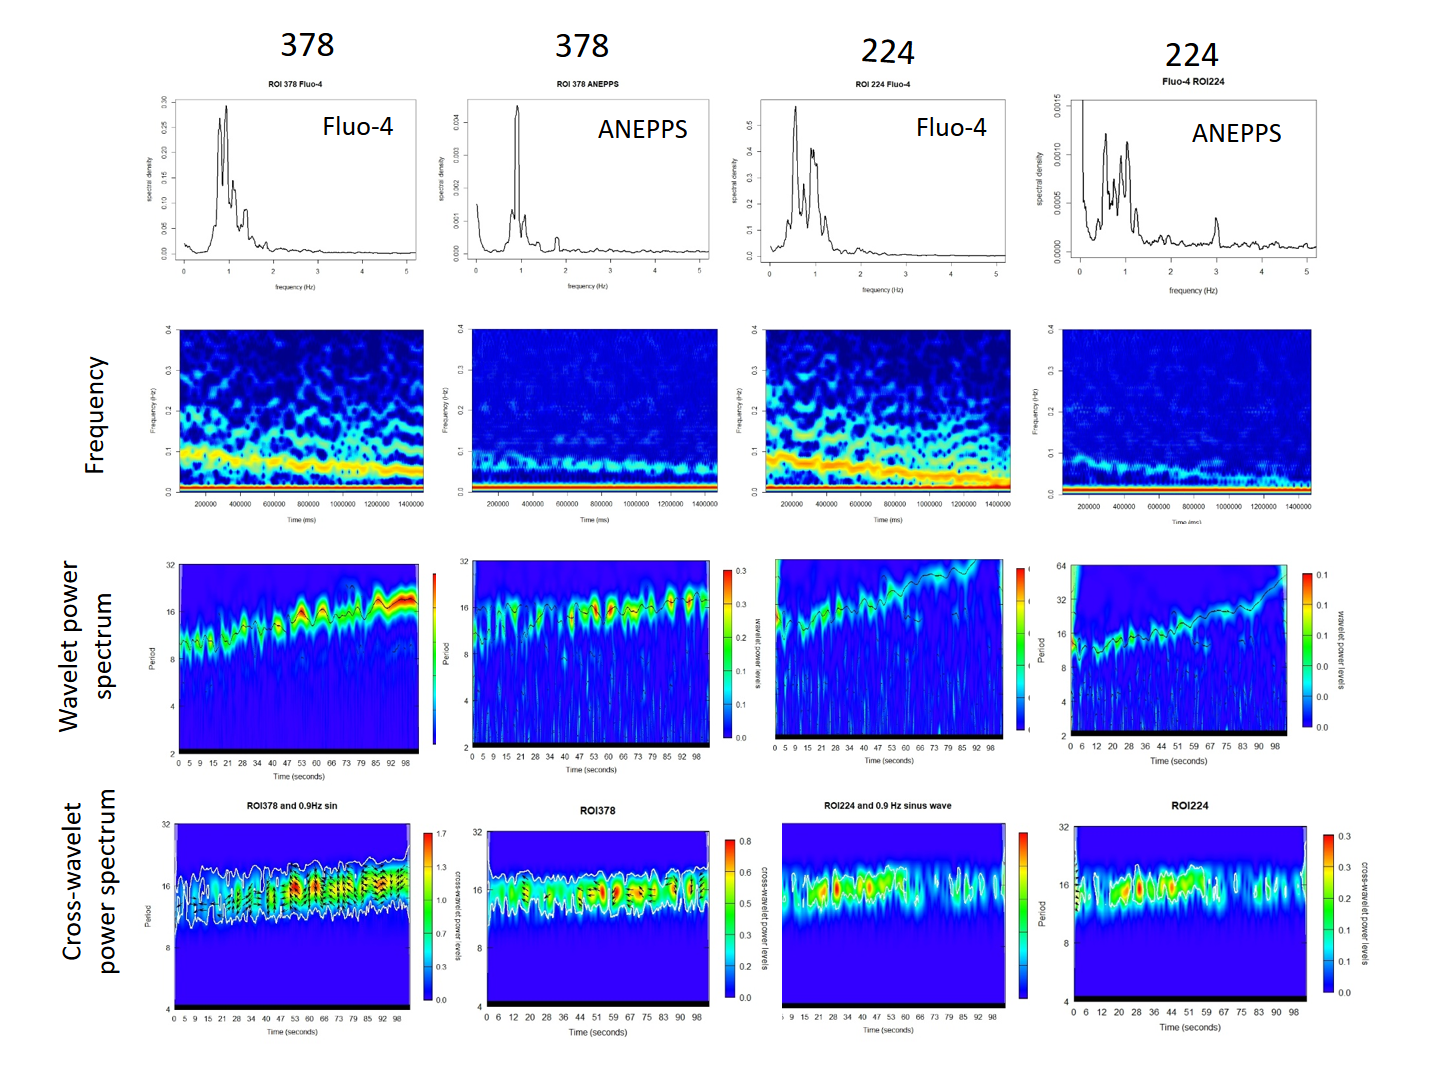
\includegraphics[width=0.9\linewidth]{fig8.png}
\caption{Simultaneous recordings of [Ca2+]i during spontaneous firing in neighboring epicardial cardiomyocytes. [Ca2+]i was monitored with the fluorescent probe Fluo-4 (see Experimental Procedures). [Ca2+]i measurement covers the 10x20 mkm ROI. AP occurred spontaneously without any stimulation}
\label{fig:fig8}
\end{figure}

We decided to apply a wavelet analysis of calcium oscillation frequencies. \cite{addison2018introduction}
norm coherence was used as a control
in cell 9, an increase in coherence is observed as the frequency decreases to the second harmonic of sinus rhythm
16 with damped low frequency oscillations
self-coherence increases in intensity and does not change in phase
cell 10 is shrinking, it can be seen on non-normalized video (see appendix)

\begin{figure}[hbt!]
\centering
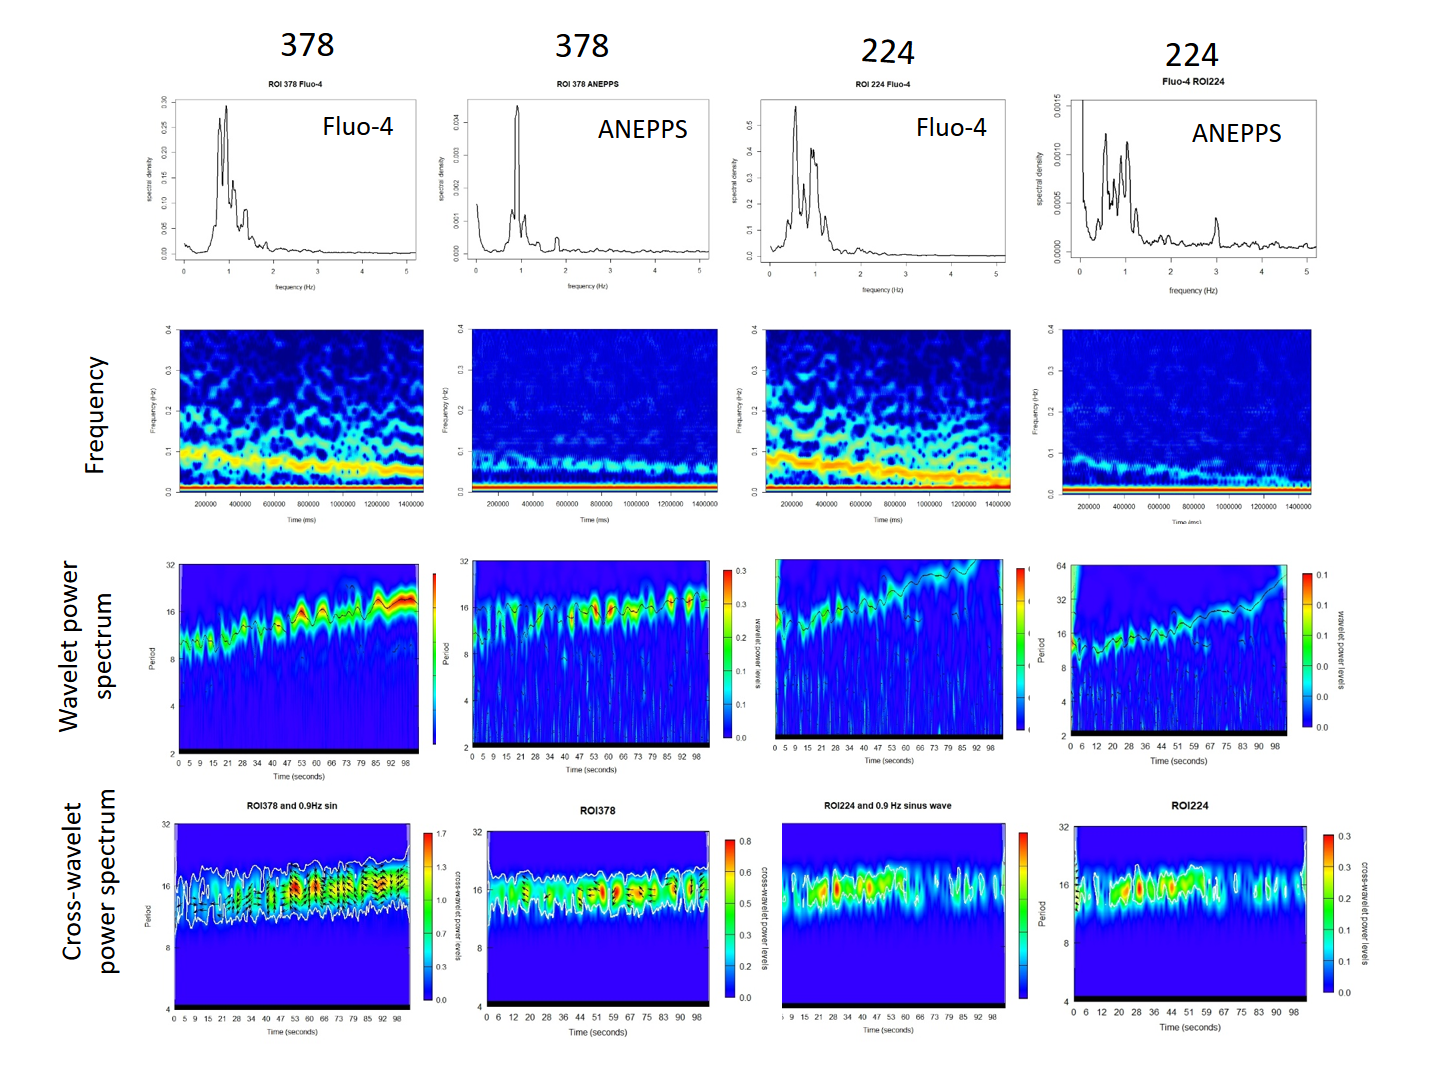
\includegraphics[width=0.8\linewidth]{fig9.png}
\caption{Wavelet coherence images of two time series provided by correspondent ROI fluorescent imaging within subepicardial layer.
The vertical axis shows the Fourier periods. The horizontal axis shows time step counts.
Further plot design options concern: plot of the cone of influence, plot of contour lines to border areas of significance, plot of the ridge, and plot of arrows to reflect phase differences.}
\label{fig:fig9}
\end{figure}


We performed a calculation of the \ref{fig:fig8} coherence between the sinus rhythm and cardiomyocytes in various stages of damage.
The role of calcium in regulation of conraction.
in the occurrence of arrhythmias.

\begin{figure}[hbt!]
\centering
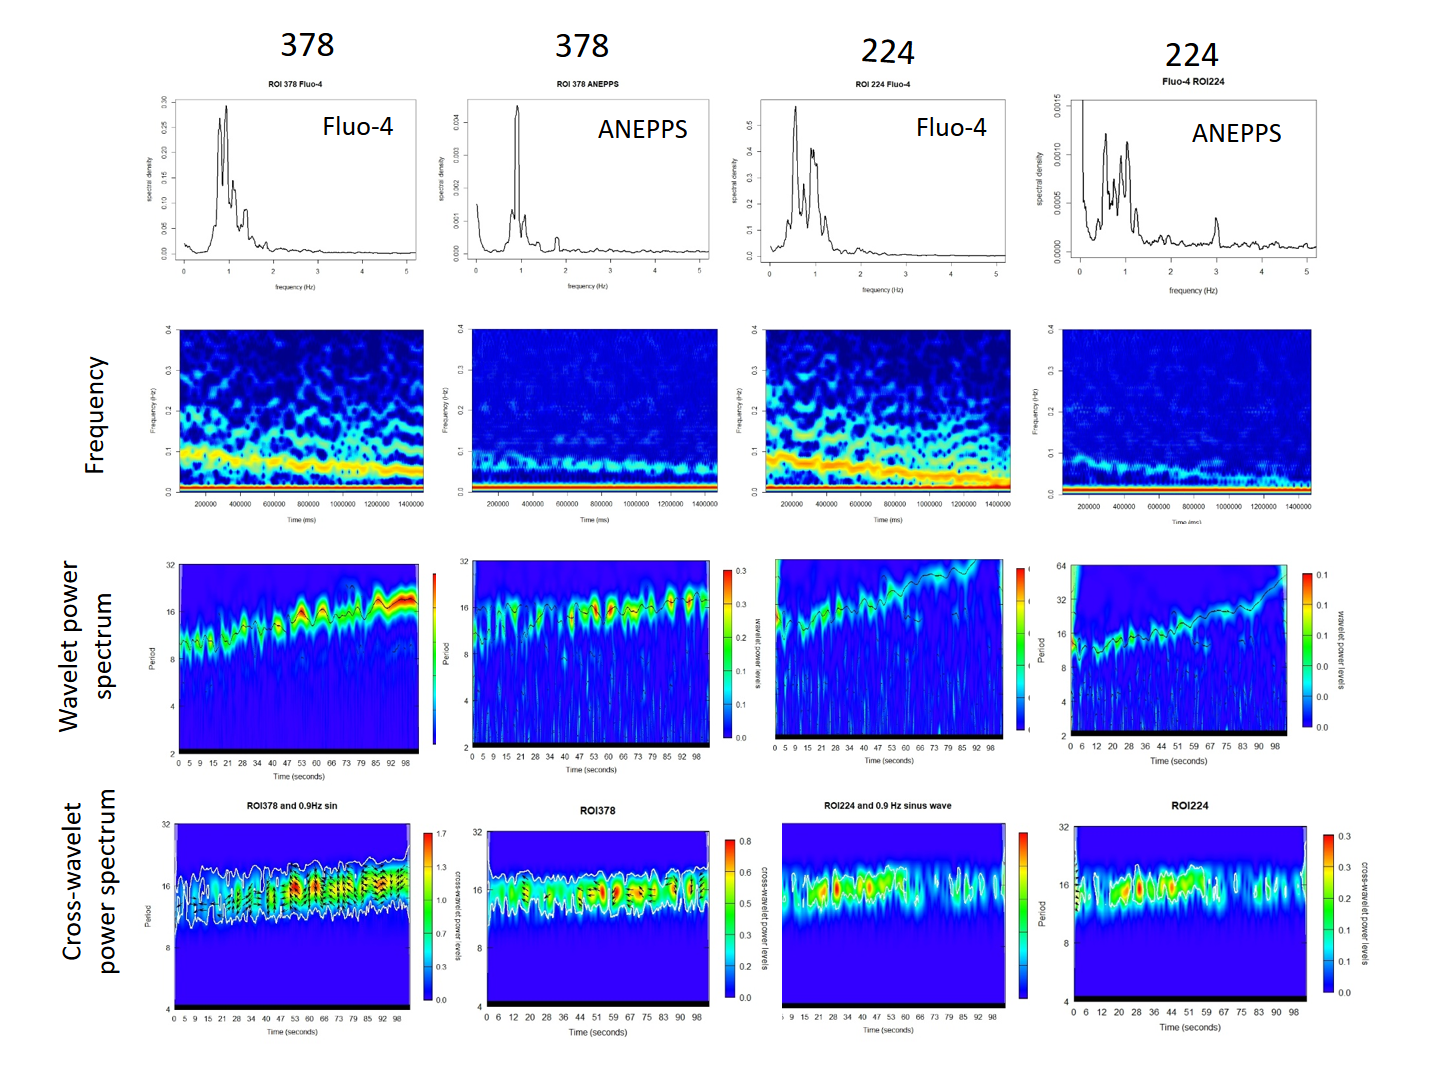
\includegraphics[width=0.8\linewidth]{fig10.png}
\caption{Wavelet coherence images of two time series provided by correspondent ROI fluorescent imaging within subepicardial layer.
The vertical axis shows the Fourier periods. The horizontal axis shows time step counts.
Further plot design options concern: plot of the cone of influence, plot of contour lines to border areas of significance, plot of the ridge, and plot of arrows to reflect phase differences.}
\label{fig:fig10}
\end{figure}


Fig. 1. Cardiomyocytes adjacent to the epicardial surface of the heart.
Based on a series of optical sections, a three-dimensional image of a portion of the myocardium of an isolated rat heart stained with a potential dependent Di-8-ANEPPS dye.
The epicardial surface of the heart is located on top.
Different types of myocardial damage.
Different parts of the myocardium of the rat, colored for active mitochondria (red) and free calcium ions (green). a is a normal tissue; b - groups of cells with reduced mitochondrial potential and elevated calcium content; c, d - groups of cells with necrotic striation. Optical sections of subepicardial ventricular layers.


The scale segments are 100 $\mu$m.
Measurement of fluorescence intensity in the area of the myocardium stained for active mitochondria (red) and free calcium ions (green).
The scale segment is 50 $\mu$m.
For comparison, six ROIs of 10 $\mu$ m x 20 $\mu$ m are selected.
Pixel intensity distribution histograms were constructed for each ROI.


In the book \cite{kockskamper2002subcellular} about atrial fibrillation ...
Arrhythmia


Fig. 11. Pairwise comparison of calcium waves of cardiomyocytes located in the perinekrozic zone of the epicardial region of the ventricular myocardium of an isolated working rat heart. Fluorescence intensity curves of Fluo-4 versus time are presented. A, B - comparison of signals in neighboring cells, C - comparison of signals in cells lying at a distance of 100 $\mu$ m from each other, D - comparison of signals in cells lying at a distance of 300 $\mu$  mfrom each other.


The FFT analysis of calcium oscillations showed that in the cardiomyocytes of the perineecrosis boundary zone, as the concentration of \ce{Ca^2+} increases, the amplitude of normal fluctuations in the concentration of ionized \ce{Ca^2+} first increases (Figure 11, A), then single calcium waves break the sinus rhythm (Figure 11, B) , then autonomous high-frequency calcium oscillations arise that attenuate, reaching a certain threshold, (Figure 11, Figure 13, Figure 13), after which the cardiomyocytes begin to hyper-shrink. Such calcium waves can be a source of arrhythmias and contribute to the development of contractile dysfunction in heart diseases.


Fig. 2.  Calcium waves in rat myocardium against a background of global calcium release.
Optical section of the epicardial region of the ventricular myocardium of the isolated working heart of the rat, painted Di-8-ANEPPS (red) and Fluo-4 (green), combined image.
The scale segment is 100 $\mu$m.
White squares indicate the selected ROI size of 100 $\mu$m x 100 $\mu$m.
Fluorescent fluorescence intensity plots in selected ROI: red line - ROI 01, green line - ROI 02.
Measurement of the fluorescence intensity versus time in the myocardium, stained for active mitochondria (red) and free calcium ions (green).
The scale segment is 20 $\mu$m. Shooting for 25 min, the frame corresponding to a point of 500 seconds is presented.
A plot of the fluorescence intensity measured in the frame is plotted against time.


Pairwise comparison of the frequencies of calcium waves of cardiomyocytes located in the perinekrozic zone of the ventricular myocardial epicardial region of an isolated working rat heart. A - comparison of signals in neighboring cells, B - comparison of signals in cells lying at a distance of 200 $\mu$m from each other
Comparison of calcium waves of cardiomyocytes located in the perinekrozic zone of the ventricular myocardial epicardial region of an isolated working rat heart. Plots of fluorescence intensity of Fluo-4 versus time are shown, which are typical for cells located at different stages of damage. The green line is a cell with a normal rhythm; blue line - a cell with a high content of Ca2 + and sinus rhythm disturbances; red line - high-frequency spindle-shaped oscillations; turquoise line - damped oscillations, cell in terminal stage; the black line is a cell in the stage of hypercontraction
Calcium waves in cardiomyocytes lying near the necrosis zone. Optical section of the myocardium stained with Fluo-4 (green) and Di-8-ANEPPS (red). On the combined image, the dotted rectangles indicate the selected ROI. The scale segment is 100 $\mu$m. On the fluorescence intensity curves of Fluo-4 in the selected ROI, damped oscillations are seen. Total observation time is 90 sec.
Optical recording of sinus rhythm in the myocardium. A - Optical sections of the epicardial region of the ventricular myocardium of the isolated working heart of the rat, painted with Di-8-ANEPPS (red) and Fluo-4 (green). B - Fluorescence intensity curves Fluo-4 (black line) and myocardial contractions (red line) versus time. Presented frames are indicated by black arrows. The scale segment is 100 $\mu$m.

Calcium waves in rat myocardium against a background of global calcium release. A - Optical sections of the epicardial region of the ventricular myocardium of the isolated working heart of the rat, painted with Di-8-ANEPPS (red) and Fluo-4 (green). B - Plots of fluorescence intensity of Fluo-4 versus time. Presented frames are indicated by black arrows. The scale segment is 100 $\mu$m.

Optical section of the myocardium stained with Fluo-4 (green).
For comparison, 12 ROIs with a size of 10 $\mu$m x 20 $\mu$m are selected.
The asterisk marks areas with necrotic striation. The scale segment is 10 $\mu$m.
Graphs of fluorescence intensity of fluo-4 versus time (left column) and the dependence of the frequency of calcium concentration fluctuations on the amplitude (right column) in the selected ROI.
Normal vibrations corresponding to sinus rhythm (ROI 1), high-frequency spindle (ROI 10), low-frequency attenuating (ROI 11) oscillations, and a signal characteristic for the cell in the stage of hyper-contraction are presented.
Calcium waves in the subepicardial myocardium in Langendorff-perfused rat heart. Fig.1. Cross-sections through image stacks acquired with laser scanning confocal microscopy of … loaded with fluo-4 and ANEPPS.


Spontaneous Ca waves in cardiomyocytes is assotioated with local damage sites.
Fig. 1 A shows a comparison of \ce{Ca^2+} levels in normal (ROI1) and locally damaged (ROI11) cells along with maximum \ce{Ca^2+} level registered from totally Ca-overloaded hypercontracted cell.

Studies were made of the frequency characteristics of calcium waves arising in cardiomyocytes of the border zone. For comparison, 12 cells were selected located next to the necrosis zone (Fig. 9). In each cell, an ROI was determined in which fluorescence fluctuation values of Fluo-4 were measured. The obtained values were processed by the FFT method in the Origin program, some of the frequency characteristics of the calcium waves are shown in Fig. 10 (the data table is presented in the file Fluo-4.
When the mitochondria and free \ce{Ca^2+} ions were stained in the absence of contractile activity and sinus rhythm (inhibition by BDM) in the heart, they were detected as areas of the normal myocardium, characterized by a high $\Delta$ $\psi$ and a low value of \ce{Ca^2+} (Fig.2, a, Fig.3, ROI 4-6), and areas of the myocardium, which is in different stages of ischemic damage.
An area was identified where, in one field of view of the microscope, it was possible to take readings from cells in successive stages of approach to death. A number of characteristics of the cells were built up, with increasing signs of ischemic damage.
For the initial stage of the lesion, groups of cardiomyocytes with a reduced and a high value of \ce{Ca^2+} are characteristic (Fig. 2b, Fig. 3, ROI 2-3). In such cells, oscillations of \ce{Ca^2+} (calcium waves) were observed. At further stages of damage in the tissue, foci of necrosis appear, which are noticeable by the appearance of necrotic striation (Fig. 2, c, d). When a normal myocardium section was observed for 25 min, a continuous decrease in the fluorescence intensity of TMRM was recorded, fluorescence intensity of Fluo-4 first increased for 15 min, and only then began to decrease (Fig. 4). These data are consistent with the notion that as the decreases, the mitochondria begin to accumulate \ce{Ca^2+}.

% By how many cells were investigated in different areas? Those graphs that you give it for individual cells? If so, it is necessary to paint each cell in detail. For example: sample 1 - intensity of the calcium signal ???, location relative to the necrosis focus ???, intensity MX ??? and all that we can say (contractility, the distribution of MX ...). Please do this for each schedule.

% In addition, you need a detailed description of each schedule. What changes specifically: amplitude, frequency, etc. Also write down in detail.

For the initial stage of damage, groups of cardiomyocytes with an elevated value of \ce{Ca^2+}, in which high-frequency calcium waves were observed (Fig. 6), are characteristic. Nascent on the edge of the cell or in its middle, these waves can spread to neighboring cells (Figure 7). With a slight increase in the intracellular calcium concentration, such waves are erased by each subsequent global calcium release (Figure 11, B), and with a strong increase in \ce{Ca^2+} in cardiomyocytes relative to the baseline observed in the normal myocardium, the global calcium release does not interfere with the formation of calcium waves (Fig. 11, B, D). Undoubtedly, the prognostic significance can be the detection of the switching point from the state of the cell, in which global waves can crush pathological, contributing to the restoration of a normal rhythm, to a transition through the "point of no return" when recovery is no longer possible.
We found that cardiomyocytes located in the border zone adjacent to the necrosis zone are characterized by an increased content of Ca2 + ions, a reduced mitochondrial potential and contractile activity. Studies were made of the frequency characteristics of calcium waves arising in cardiomyocytes of the border zone. For comparison, 12 cells were selected located next to the necrosis zone (Fig. 9). In each cell, an ROI was determined in which fluorescence fluctuation values of Fluo-4 were measured. The obtained values were processed by the FFT method in the Origin program, some frequency characteristics of the calcium waves are shown in Fig. 10 (the data table is presented in the file Fluo-4 ROI 01-12.xlsx
The FFT analysis of calcium oscillations showed that in the cardiomyocytes of the perineecrosis boundary zone, as the concentration of Ca2 + increases, the amplitude of normal fluctuations in the concentration of ionized Ca2 + first increases (Figure 11, A), then single calcium waves break the sinus rhythm (Figure 11, B) ,
then autonomous high-frequency calcium oscillations arise which, attaining a certain threshold, decay (Figure 11 B, D, Figure 12, Figure 13), after which the cardiomyocytes begin to hyper-shrink. Such calcium waves can be a source of arrhythmias and contribute to the development of contractile dysfunction in heart diseases.
The cardiomyocytes adjacent to the necrosis zone were characterized mainly by slow, damped calcium waves with a large amplitude (Fig. 8).

\begin{description}
\item[Word] Definition
\item[Concept] Explanation
\item[Idea] Text
\end{description}

An example quotation:

\begin{quote}
Lorem ipsum dolor sit amet, consectetur adipiscing elit, sed do eiusmod tempor incididunt ut labore et dolore magna aliqua. Ut enim ad minim veniam, quis nostrud exercitation ullamco laboris nisi ut aliquip ex ea commodo consequat.
\end{quote}


\section*{Discussion}

\cite{bonilla2019enhancement} provide the first demonstration of local, transient \ce{Ca^2+} entry
(LoCE) events, which comprise cardiac SOCE. Although infrequent in WT myocytes, LoCEs occurred
with greater frequency and amplitude in CpVt myocytes.

As was clearly demonstrated \cite{matsuura2018intravital},
Ischemic myocardial damage manifests itself as a source of calcium waves.
We show in this paper, on a model of an isolated rat heart, what a the frequency characteristics of calcium oscillations recorded in the border zone near necrosis.
Intracellular calcium accumulation caused by weakening of ATP-dependent mechanisms due to lack of oxygen supply causes foci of high-frequency calcium oscillations that go out of control by sino-atrial thythm.

scale modeling approach that spans from single channel to whole-cell and spatial
simulations, we show that both CICR and SOICR gating modes can indeed activate RyR2 channels and modify \ce{Ca^2+} spark dynamics in a manner consistent
with experimental observations. However, detailed comparison of \ce{Ca^2+} wave
generation and CRU-to-CRU \ce{Ca^2+} wave propagation shows that CICR alone
is a sufficient, and necessary, mechanism to explain Ca2þ release in heart under
both physiological and pathological conditions
\cite{williams2017does}

We assume that such high-frequency activity may cause arrhythmias.

In the ischemic myocardium \ce{Ca^2+} waves are regarded as arrhythmogenic substrates.
To quantitatively image how \ce{Ca^2+} waves interfere with \ce{Ca^2+} transients from spontaneous sinus rhythm we used a single-photon confocal laser scanning microscopy in Langendorff-perfused rat hearts.
This technique has allowed Intravital imaging visualization of \ce{Ca^2+} waves propagation at the single-cell level in epicardial cardiomyocytes, avoiding the damage induced by isolation of cardiomyocytes.
The effects of hypoxia on oscillations in intracellular calcium concentration \ce{Ca^2+} were determined in isolated rat heart.
The aim was to investigate the frequency characteristics of calcium oscillations arising in the epicardium in response to ischemia
Spectral  analysis of myocardial analysis of calcium oscillations in rat heart using confocal microscopy was carried out.
Optical recording of calcium currents in the rat myocardium during the development of ischemic injury.
In cells located at the periphery of the lesion focus, the basal level of calcium remains within normal limits, point-like, prismatic wave sources appear that do not extend to the cell as a whole and are extinguished by a wave of normal ejection.
A wave of normal ejection is the result of the work of the pacemaker cells and is accompanied by a synchronous muscle contraction.
In cells closer to the lesion focus, the calcium concentration rises.
Microtraumas, points of damage are sources of waves.
As a result of the hyperscrubbing of ischemic cells, there are gaps between the cardiomyocytes that become the sources of individual transverse waves that cover the whole cell and are able to spread to neighboring cells.
As a result of interference of several calcium waves, wave packets arise, the amplitude of which increases as the intracellular concentration of free calcium ions increases.
An arrhythmia arises, representing a group of partially damaged and contiguous intact myocardial cells characterized by an elevated concentration of free calcium ions that have their own rhythms of calcium release and muscle contractions and are not affected by pacemaker cells.
and during the detachment of the cell the frequency increases spasmodically.
Intracellular calcium waves were intensively studied in isolated cardioiocytes by the linescan method (Gyorke, Sunil Kapur).
The results obtained revealed the large role of calcium sparks in the nucleation of these waves.
Spectral analysis of
 measure the intensiy of Systolic \ce{Ca^2+} alternans
hypercontracture-indused calcium oscillations interfere with Systolic \ce{Ca^2+} alternans
SR \ce{Ca^2+} content changes during alternans \cite{diaz2004sarcoplasmic}
We assume that high-frequency calcium oscillations arise at the time of cardiomyocyte damage caused by hypercontraction.
Since in the course of hypercontraction initial damage can be localized as two adjacent sarcomeres,
Propagation of transverse calcium wave along longitudinal axis
Such anisotropic protagation of calcium waves was described in 1994 by Engel et al, and velocity of wave propagation rise with temperature.
Formation of calcium waves of different type in isolated cardiac myocytes \cite{ishida1999formation}
that this type of calcium waves initiate from stochastic \cite{izu2001evolution} subdiffusive  \cite{chen2014ryanodine} Chen et al  calcium sparks.
This propagation pattern was satisfactorily explained by Finite-element simulations of the three-dimensional cell model, conducted for different intracellular locations of triggering calcium sparks \cite{tracqui2009integrated}
we observed for 100 sec Sustained transverse calcium wave patterns in epicard of isolated heart
for some time the damaged cardiomyocyte, which has not lost its connection with neighboring cells, can be a source of high-frequency calcium waves, which are transmitted to neighboring cells through gap junctions.
Tomoyuki at al using confocal device with simultaneous recording of electrocardiograms demonstrated that \ce{Ca^2+} waves in Langendorff-perfused rat hearts were completely abolished by ventricular excitation, and that under highly \ce{Ca^2+} -overloaded conditions \ce{Ca^2+} waves may occur more frequently and propagate more prevalently to the surrounding cells. Authors suggested that \ce{Ca^2+} waves play little, if any, pathophysiological role (6,7). Later, it was established that myocardial injury induces \ce{Ca^2+} waves in the heart (8,9). Baader et al proposed that spatio-temporal summation of changes in membrane potential caused by individual \ce{Ca^2+} waves may underlie the generation of triggered electrical ectopic impulses (10).
In recent years, it has become apparent that myocardial ischemia can cause ventricular arrhythmias and sudden cardiac death.
Time series
Analysis of oscillation periodicity reveal
Wavel coherence analysis of calcium oscillation reveal...
Wavelet transform coherence (WTC) is a method for analyzing the coherence and phase lag between two time series as a function of both time and frequency (\cite{chang2010time}).


Wavelet toolbox is a useful tool to study hyperscanning data. Many recent publications on NIRS hyperscanning use wavelet coherence to quantify the relationship between two interacting brains (e.g. Baker et al 2016, Nozawa et al 2016). You can see more information about wavelet coherence at \href{http://www.alivelearn.net/?p=1169}{site}.

In the above figure, I plot the wavelet coherence between the two signals in both time and frequency domain. Coherence is kind of correlation. 1 (red) means the two signals are highly correlated and 0 (blue) means no correlation. There are definitely something interesting between the two signals.

First, there is a red band in the period 8 region. As the sampling frequency of the signals is 10Hz, period 8 means 0.8s. This band is originated from heart beating (~1Hz) and indicates that the two people’s heart beating is highly correlated.

Second, there are some red blobs in the period 64 region. The button pressing is occurring at 6-7s frequency. These blobs indicate that the two people’s brain are correlated during button pressing.

So, with wavelet coherence analysis, you can discover something you might not discover with other methods.

In the following examples, I created two time series, x (blue) and y (red) with different properties (phase shift, frequency and amplitude) and run wtc(x,y,’mcc’,0) command. Small white noise was added to the time series.

1. Phase shift and angle.
A rightward arrow indicates 0 lag; a bottom-right arrow indicates a Small


Dissinchrony
Alternans
Hypoxia
Frequency
Cardiac
Heart imaging
Repolarization
Propagation
Release
Measurements
Dynamics
Changes
Information
Arrhythmia
Arrhythmogenic
Ectopic
Myocardial alternans
Increase
Experimental
Motion time
Mitochondrial
Radiation of aberrant signal
Noise
Oscillations
Stochastic calcium Oscillations
Phenomenon
This resulted in
 during the repolarization phase,
thus further increasing APD and \ce{Ca^2+} loading. This positive-feedback loop led to EADs and
ultimately failure to repolarize. It is possible that the saturating behavior of LCC \ce{Ca^2+}-dependent activation in this model prevents sufficient LCC inhibition required for repolarization in
the presence of elevated SR \ce{Ca^2+}
The LCC model also does not incorporate “global” \ce{Ca^2+}
sensing , which would inhibit LCC openings in the presence of sustained elevated \ce{Ca^2+}.
Future work is needed to understand the contributions of these mechanisms, as they may
affect the conditions under which the model exhibits DADs during pacing.The distribution of DADs was controlled by both \ce{Ca^2+} and \ce{Ca^2+}SR. This was revealed
by the apparent change in the threshold SR \ce{Ca^2+} load for spontaneous \ce{Ca^2+} wave formation
during pacing (see Fig 3). Elevated diastolic \ce{Ca^2+} increased RyR opening rate and thus perpetuated \ce{Ca^2+} wave formation at lower SR \ce{Ca^2+} loads. It also caused more rapid loading of the
SR to induce overload. Cellular \ce{Ca^2+} loading also increased the amplitude of DADs due to the
greater number and concurrence of \ce{Ca^2+} wave nucleation sites, which is in agreement with
A significant contribution of this work is that the emergence of sudden arrhythmias can be
causally linked to stochastic molecular events. A computationally efficient method was developed to estimate the probability of extreme DADs. An important assumption of this method is that the spontaneous \ce{Ca^2+} release events in neighboring cells are decoupled.
It is known that membrane depolarization increases the frequency of \ce{Ca^2+} waves by reducing NCX-mediated
\ce{Ca^2+} efflux and thus promoting \ce{Ca^2+} waves due to increased intracellular \ce{Ca^2+} \cite{walker2017estimating}.
In the present study we visualized precise \ce{Ca^2+} dynamics of atrial myocytes in the perfused rat heart.
By using the in situ rapid confocal imaging system
we found that in Langendorff-perfused rat heart has to show
spatiotemporally \ce{Ca^2+} dynamics especially According to

\iffalse
our \ce{Ca^2+} dynamics studies to date [9, 11, 25], such nonuniformity
in the \ce{Ca^2+} transients was not predominantly
observed in intact ventricles, and the observed features in
the atrial \ce{Ca^2+} dynamics would partly be related to the
structural difference, i.e., paucity of t-tubules.

\fi

In principle, individual atrial myocytes in the perfused hearts showed spatiotemporally uniform \ce{Ca^2+} dynamics with frequency-dependent abbreviation of \ce{Ca^2+}-transient durations,
a confirmation of the atria being a functional syncytium (Fig. 2).
However, even under apparently intact Langendorff perfusion,
individual myocytes often exhibited spatially non-uniform \ce{Ca^2+} dynamics,
e.g., cluster-like rises of \ce{Ca^2+}, wave-like propagation of \ce{Ca^2+},
and beattobeat variability of durations and amplitude alternans of \ce{Ca^2+} transients,
all of which emerged on excitation instead of uniform \ce{Ca^2+} transients (Figs. 3 and 4).
\cite{jiang2014pacing}, \cite{aguirre2014intravital}
Spontaneous \ce{Ca^2+} waves during diastole are indicative of cellular Ca 21 overload \cite{macquaide2007measurement}

%\begin{figure}
%    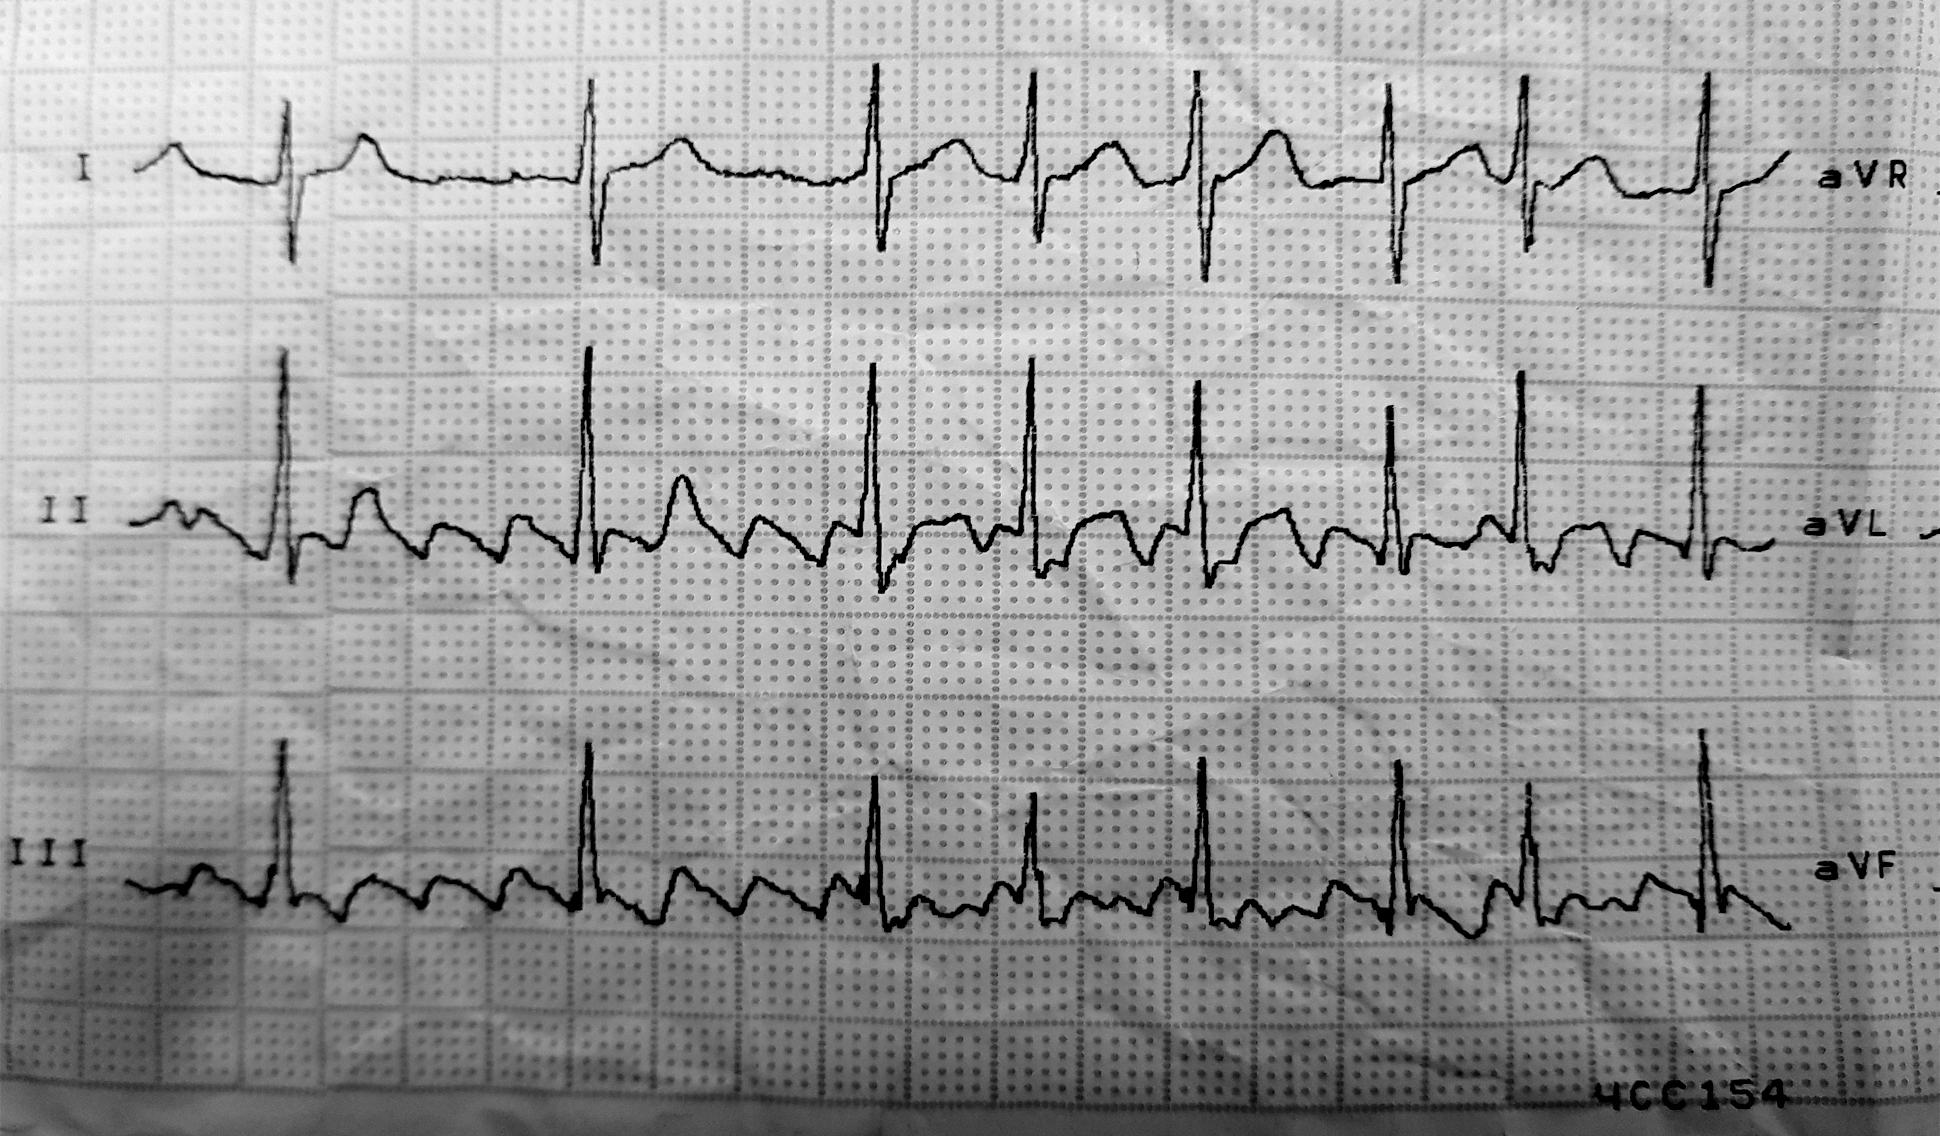
\includegraphics[width=0.6\linewidth]{figA.jpg}
%    \caption{Arrhythmia}
%    \label{fig:figA}
%\end{figure}

Analysis of calcium alternans in ischemic condition
calcium overloading
cardiac function.
spectrum

Spectral analysis of hypoxia-indused calcium waves in isolated rat heart on the subcellular level
Spontaneous calcium oscillations in unstimulated heart muscle
Local hypercontracture induces hight-frequency calcium oscillations

And they saw there that over time the frequency of high-frequency waves decreases, and it’s in cells that are gradually hyper-reduced, apparently.

The decrease in the frequency of oscillations in time is shown.
if it is damaged cells that are in the process of over-contraction
are the source of oscillations
\cite{sato2014depolarization}
citation \cite{sato2014depolarization}.

Short Time Fourier Transform (STFT) analysis provides information about the number of oscillators, but its time resolution is limited.
Wavelet tranform allows analysis of non-stationary signals.

The presented results of wavelet tranform of obtained oscillation time dependencies confirmed the presence of two? harmonic components in each...
and allowed more accurate visualization of the frequency changes in time.

Thus, for the ...

\section*{Conclusion}

Sed ut perspiciatis unde omnis iste natus error sit voluptatem accusantium doloremque laudantium, totam rem aperiam, eaque ipsa quae ab illo inventore veritatis et quasi architecto beatae vitae dicta sunt explicabo.
Understanding these mechanisms will help to further protect the heart muscle during cardiac surgery and in the long run will improve the prevention of heart disease.

\section*{Author Contributions}

Author2 designed the research. Author1 carried out all simulations, analyzed the data. Author1 and Author2 wrote the article.

\section*{Acknowledgments}

We thank Dr. Polyanski , B. Harper, and J. Doe for their help.

% Uncomment if using bibtex (default)
\bibliography{mybib}

% Uncomment if using biblatex
% \printbibliography

\section*{Supplementary Material}
An online supplement to this article can be found by visiting BJ Online at \url{http://www.biophysj.org}.

\subsection*{ImageJ macros}\label{macros}
\begin{lstlisting}
x = 1;
y = 1;
width = 20;
height = 20;
spacing = 1;
numRow = 24;
numCol = 24;
u
for(i = 0; i < numRow; i++)
{
	for(j = 0; j < numCol; j++)
	{
		xOffset = j * (width + spacing);
		print(xOffset);
		yOffset = i * (height + spacing);
		print(yOffset);
		makeRectangle(x + xOffset, y + yOffset, width, height);
		roiManager("Add");
		if (roiManager("count") > 1000)
			{
			print("Maximum reached: 1000 entries have been created.");
			exit;
			}
	}
}
\end{lstlisting}

\subsection*{R code}

\begin{lstlisting}[language=R]

# Calcium oscillations analysis, 2019

options('stringsAsFactors' = FALSE)
library(WaveletComp)
library(phonTools)
library(seewave)
library(ggplot2)
library(ggpubr)
library(dplyr)
library(xlsx)

#-----import constats-----
s.rate <- 14.142211 #
del <- 0.0707103 # frame duration in seconds
fsin <- 0.9025023 # Hz, sinus rythm main frequency
# fsin <- 1 # 1 Hz sin wave frequency
fs <- 14.142211 # samples per second
df <- 1/fs # seconds per second
stoptime <-  110.803 # signal length in seconds
# Insert your specification of the time axis:
index.ticks  <- seq(0, 1567, by = 1) # 1567 is signal frame count
index.labels <- seq(0, 1567, by = 1)*103.803/1567
index.labels.rounded <- round(index.labels, 0)

t <- seq(0, stoptime, by = df)
sinwave <- sin(2*pi*fsin*t)

plot(t, sinwave, type = 'l',
     main = "Sinus wave",
     xlab = 'Time, sec', ylab = 'value',
     xlim = c(20, 80), ylim = c(-1, 1))


sinwave_complex <- c(sin(2*pi*1*t)[1:500],
                     sin(2*pi*2*t)[501:1000],
                     sin(2*pi*3*t)[1001:1567])

# Load data from ImageJ BAR Time series analisys
# calcium <- read.csv('fluo.csv', sep = ',') # Fluo-4 raw
calcium <- read.csv('fluoF0.csv', sep = ',') # Fluo-4 F0 normalazed signal
# calcium <- read.csv('anepps.csv', sep = ',') # Di-8-ANEPPS raw
calcium <- read.csv('aneppsF0.csv', sep = ',') # F0 normalazed signal
colnames(calcium)[1] <- "frame" # rename first column

calcium <- read.csv('fluoPxF0.csv', sep = ',')
colnames(calcium) <- c('frame','ROI512x512','ROI180x40',
                      'ROI40x40', 'ROI2x2', 'ROI10x10')

calcium <- read.csv('fluoF0-roi123.csv', sep = ',')
colnames(calcium) <- c('frame','ROI20x20','cell', 'ROI512x512')
#------------------------------------------
# Calibrate time: 110.803 sec / 1567 frames
calcium$time <- calcium$frame * 110.803 / 1567
# Add sin waves
calcium$sin <- sinwave
calcium$sincomp <- sinwave_complex
#--------------------------
# Select ROI from 20x20 ROI grid
xcal <- calcium$ROI20x20 # from Y0 to Y575 = ROI1 to ROI576

#--------------------------
# time series analysis
calcium_ts <- ts(xcal, start = calcium$time[1])

x.spec <- spectrum(calcium_ts, log = "no", span = 10, plot = FALSE)
spx <- x.spec$freq/del
spy <- 1*x.spec$spec

plot(spy ~ spx, xlab="frequency (Hz)", ylab="spectral density",
     type="l", lwd = 2, main = 'ROI ', xlim=c(0,5))
#_______________________________Fluo-4____D-8-ANEPPS
# A Test Signal Containing Four Sequential Sinusoids

# Peaks detection

fpeaks(spec(calcium_ts, f=s.rate), nmax = 10,
       threshold = 0.5,
       plot = T,
       title = TRUE,
       xlab = "Frequency (Hz)", ylab = "Amplitude",
       labels = TRUE, legend = TRUE, digits = 2)*1000

peaks <- fpeaks(spec(calcium_ts, f=s.rate), nmax = 10,
                threshold = 0.5,
                plot = T,
                title = TRUE,
                xlab = "Frequency (Hz)", ylab = "Amplitude",
                labels = TRUE, legend = TRUE, digits = 2)*1000
# write.csv2(peaks, file = 'norm_ROI1_Fluo4_peaks.csv')

#>>>>>>>>>>>>>>>>>>>>>>>>>>
# Frequency
spectrogram(calcium_ts, 14.29745, windowlength = 95000, 0.01,
            timestep = 1000,
            maxfreq = 0.4,
            colors = TRUE,
            dynamicrange = 40, nlevels = dynamicrange, maintitle = "",
            show = TRUE, window = 'hamming',
            quality = TRUE)

#>>>>>>>>>>>>>>>>>>>>>>>>>>
# Period
my.data <- data.frame(x = calcium_ts)
my.w <- analyze.wavelet(my.data, "x",
                        loess.span = 0,
                        dt = 1,
                        dj = 1/500,
                        lowerPeriod = 2,
                        upperPeriod = 32,
                        make.pval = TRUE, n.sim = 10)
## Insert your specification of the time axis
# "interval" or "i": equidistant breakpoints
# (from 0 through maximum value)
wt.image(my.w, color.key = "i", # or use 'quantile' key
         n.levels = 250, max.contour.segments = 10000,
         useRaster = TRUE, plot.contour = FALSE,
         legend.params = list(lab = "wavelet power levels"),
         periodlab = "Period", timelab = "Time (seconds)",
         spec.time.axis = list(at = index.ticks, labels = index.labels.rounded))


#^^^^^^^^^^^^^^^^^^^^^^^^^^^
# Wavelet coherency


x <- sinwave
y <- calcium_ts
# y <- ts(calcium$sin, start = calcium$time[1])
# x <- ts(calcium$Y554, start = calcium$time[1])
my.data <- data.frame(x = x, y = y, date = calcium$time)
my.wc <- analyze.coherency(my.data, my.pair = c("x", "y"),
                           loess.span = 0,
                           dt = 1,
                           dj = 1/100,
                           lowerPeriod = 4, upperPeriod = 32,
                           make.pval = TRUE, n.sim = 10)

wc.image(my.wc, n.levels = 250, color.key = "interval",
         siglvl.contour = 0.1, siglvl.arrow = 0.05, which.arrow.sig = "wt",
         legend.params = list(lab = "cross-wavelet power levels"),
         label.time.axis = TRUE,
         main = "ROI512x512 and 0.9Hz sinus wave",
         periodlab = "Period", timelab = "Time (seconds)",
         spec.time.axis = list(at = index.ticks, labels = index.labels.rounded))
#^^^^^^^^^^^^^^^^^^^^^^^^^^^


# Remove outliers function

outliers.rm <- function(x)
{
        q <- quantile(x, probs = c(0.25, 0.75))
        q <- unname(q)
        for (i in x)
        {
                if ( i < q[1] - 1.5*IQR(x) ||
                     i > q[2] + 1.5*IQR(x)) {
                        x <- x[x != i]
                        return(x)
                }
                else {
                        return(x)
                }
        }
}

# This function extracts frequencies from time-series data
# and remove outliers (save to frequencies.rm)

myfreq <- function(x) {
        s.rate <- 14.142211 # samples per second
        df <- 1/s.rate # seconds per second
        mypeaks <- data.frame()
        calcium <- read.csv(x, sep = ',')
        colnames(calcium)[1] <- "frame" # rename first column
        calcium$time <- calcium$frame * 110.803 / 1567
        l <- length(colnames(calcium))-2
        mydata <- data.frame(matrix(ncol = 2, nrow = 0))
        colnames(mydata) <- c("ROI", "freq")
        for (i in 1:l){
                tryCatch({
                        roi <- paste('Y', as.character(i-1), sep="")
                        calcium_ts <- ts(calcium[,roi], start = calcium$time[1])
                        peaks <- fpeaks(spec(calcium_ts, f=s.rate),
                                        nmax = 20, threshold = 0.5, # set nmax for peaks quantity
                                        plot = FALSE, title = FALSE,
                                        mel = FALSE, legend = FALSE,
                                        labels = FALSE)*1000
                        df <- data.frame('ROI' = roi,
                                         'freq' = matrix(unlist(peaks[,"freq"]),
                                                         nrow=length(peaks[,"freq"]), byrow=T))
                        mydata <- rbind(mydata, df)
                }, error=function(e){cat("ERROR :",conditionMessage(e), "\n")})
        }
        frequencies <<- mydata
        mydata.rm <- data.frame(matrix(ncol = 2, nrow = 0))
        colnames(mydata.rm) <- c("ROI", "freq")
        for (i in 1:l){
                tryCatch({
                        roi <- paste('Y', as.character(i-1), sep="")
                        df.rm <- data.frame('ROI' = roi,
                                            'freq' = outliers.rm(frequencies[frequencies$ROI==roi,]$freq))
                        mydata.rm <- rbind(mydata.rm, df.rm)
                }, error=function(e){cat("ERROR :",conditionMessage(e), "\n")})
        }
        frequencies.rm <<- mydata.rm
}


#--------------------------

\end{lstlisting}

\subsection*{Video files}

calcium-waves-Fluo-4-ANEPPS-10fps.wmv

094Roi.avi

\subsection*{Tables in csv format}

calcium.csv

094px.csv

\iffalse
А не посчитать ли дифференциальное уравнение, декремент затухания?..
причина затуханий - сокращение клетки?
\fi

\end{document}
